\RequirePackage{plautopatch} % pLaTeX / upLaTeX / LuaTeX-ja の不具合修正など
\documentclass[a4paper,10.5pt]{ltjsarticle}
\usepackage{luatexja}        % LuaTeX-ja で日本語を扱う

% -------------------------------
% フォント関連の設定
% -------------------------------
\usepackage{luatexja-fontspec}

% -------------------------------
% 数式・数理フォントパッケージ
% -------------------------------
\usepackage{amsmath}
\usepackage{amssymb}          % \mathbb などを使用可能に

% -------------------------------
% 図を生成するためのパッケージ
% -------------------------------
\usepackage{tikz}
\usepackage{pgfplots}
\pgfplotsset{compat=newest}
% -------------------------------
% 表を生成するためのパッケージ
% -------------------------------
\usepackage{booktabs}
\usepackage{array}
\usepackage{mathptmx}
% -------------------------------
% よく使われるパッケージ群
% -------------------------------
\usepackage{geometry}
\usepackage{multicol}
\usepackage{titlesec}
\usepackage{tocloft}
\usepackage{caption}
\usepackage{flushend}
\usepackage{graphicx}
\usepackage{here}
\usepackage{subfig}
\usepackage{multirow}
\usepackage{threeparttable}
\usepackage{tabularx}
\usepackage{enumitem}
\usepackage{url}
\usepackage{tabularx}
\usepackage{subcaption}
\usepackage{indentfirst}

% -------------------------------
% 用紙余白等の設定
% -------------------------------
\geometry{
  top=20mm,
  bottom=20mm,
  left=20mm,
  right=20mm
}

\setlength{\baselineskip}{14pt}  % 行間

% -------------------------------
% タイトルやセクション見出しのフォーマット
% -------------------------------
\titleformat{\section}
  {\large\bfseries}
  {\thesection.}
  {1\zw}{}

\titleformat{\subsection}
  {\large\bfseries}
  {\thesubsection.}
  {1\zw}{}

\titleformat{\subsubsection}
  {\large\bfseries}
  {\thesubsubsection.}
  {1\zw}{}

\titlespacing*{\section}{0em}{1em}{1em}
\titlespacing*{\subsection}{0em}{1em}{1em}
\titlespacing*{\subsubsection}{0em}{1em}{1em}

% -------------------------------
% 目次の設定
% -------------------------------

\setcounter{tocdepth}{3}          % 目次の深さ
\makeatletter
\renewcommand{\numberline}[1]{#1.~}
\renewcommand{\cftsecleader}{\cftdotfill{\cftdotsep}}
\renewcommand{\cftsubsecleader}{\hfill}
\renewcommand{\cftsubsubsecleader}{\hfill}
\cftpagenumbersoff{subsection}
\cftpagenumbersoff{subsubsection}
% (例) section, subsection, subsubsection のインデントを調整
\cftsetindents{section}{0em}{5em}
\cftsetindents{subsection}{1em}{5em}
\cftsetindents{subsubsection}{1.5em}{5em}
\makeatother

% キャプション(図表の見出し)フォントサイズ設定
\DeclareCaptionFont{designatedFont}{\fontsize{10.5pt}{14pt}\selectfont}
\captionsetup{labelsep=space} % コロンを削除し、スペースに変更


% -------------------------------
% タイトル情報
% -------------------------------
% \title{サンプル論文タイトル}
% \author{山田 太郎}
% \date{\today}


\begin{document}

% \maketitle
% \thispagestyle{empty}
% \clearpage

\tableofcontents
\thispagestyle{empty}



% ******************************************************
% 1. はじめに
% ******************************************************
\clearpage
\setcounter{page}{1}
\section{はじめに}

\subsection{研究の目的と方法}

%何をしたか
%背景
近年, 小型無人航空機(ドローン)の研究開発が活発に進められており, 物流, 災害対応, 農業など多岐にわたる分野での活用が期待されている. 
特に複数のドローンを協調させる編隊飛行技術の発展により, 大規模な空中ネットワークの構築が可能となり, 映像の中継伝送や災害時のバックアップネットワークの迅速な展開が実現しつつある. 
しかしドローンが飛行する空中環境では自由空間伝搬の特性により, 電波干渉が深刻な問題となる. 
障害物が存在しないため信号の減衰が少なく, 中継先を超えて他のドローンへ不要な電波が到達するオーバーリーチ干渉が発生しやすい. 
特に直線的な中継伝送ではこの影響が顕著となり, 通信効率の低下を招く. 
この問題を解決するために, 直線に配置されたドローン中継伝送におけるオーバーリーチの問題を抑制するCTR(Cooperation Through Relay)方式が提案されている.
本方式では, 送信信号の届く中継局まで一度の通信で中継することで, 自由空間伝搬損失を逆手に取り, 中継のオーバーヘッドおよびオーバーリーチ干渉を削減する. 
本研究では, 提案手法において干渉/誤りが生じた際と生じない際で従来方式及びCTR方式でそれぞれのスループット特性計算した.
誤りが生じない際には, 中継局をスルーすることによるCTR方式の効果を評価し, スループット特性を比較した.
また, 誤りが生じた際には, 誤り率を変化させたときのスループット特性を評価・比較した.

\subsection{本稿の構成}
本稿の構成は以下のとおりである.
第2章では, 計算手法について説明する.
第3章では, 従来方式の概要を述べる.
第4章では, 提案手法であるCTR方式について説明する.
第5章では, 従来方式とCTR方式の評価および比較及び評価をする.
第6章 は, 本研究の結論と今後の課題について述べる.

% ******************************************************
% 2. 計算手法
% ******************************************************
\clearpage
\section{計算手法}
CTR方式の性能を評価するために用いた計算手法について詳述する。

\subsection{無線LANシステムにおける変調方式と伝送レート}
本節では無線LANシステムにおける変調方式と伝送レートの関係と,伝送レートと伝送距離の関係についてIEEE802.11gを例に説明する.
無線通信では送受信局が通信に使用する伝送速度の定義があり,通信時にはこれに基づいて伝送レートを決定する.\par
表\ref{tab:IEEE802.11g_TR&Modulation} にIEEE802.11gで使用される変調方式・符号化率と最低受信感度($R_{\text{min}}$) および伝送レート(TR) の関係を示す.
無線LANの伝送速度は変調方式と符号化率の組み合わせによって決まり,11gのOFDMを用いた伝送レートは6Mbpsから54Mbpsまでの8つの伝送レートが定義されている.
各伝送レートごとに最低受信感度が定められており,これは受信局が受信できる最小の電力を示し,それ以下の受信電力ではその伝送レートを使用できない.
例えば伝送レートが54Mbpsの最低受信感度は-65dBmとなっており,受信局の受信電力が-66dBmの場合は,最低受信感度の-65dBmを下回るため,フレームを受信することができない.
また,変調方式の多値化と符号化率を上げることで,より高いSNR(Signal to Noise Ratio)を必要とする.必要とされるSNRと$R_{\text{min}}$の関係は
\begin{equation}
  SNR = R_{\text{min}} + 85[dB]
\end{equation}
と表される.ここで,SNRは受信電力と雑音電力の比である.

\begingroup
\setmainfont{Times New Roman} 
\begin{table}[h]
  \caption{IEEE802.11gで使用される変調方式・符号化率と最低受信感度($R_{\text{min}}$)および伝送レート(TR)の関係}
  \centering
  \renewcommand{\arraystretch}{1.5}
  \begin{tabular}{c c c c}
    \toprule
    TR [Mbps] & Modulation & Coding & $R_{\text{min}}$[dBm] \\ 
    \midrule
    6  & BPSK  & 1/2  & -82 \\
    9  & BPSK  & 3/4  & -81 \\
    12 & QPSK  & 1/2  & -79 \\
    18 & QPSK  & 3/4  & -77 \\
    24 & 16QAM & 1/2  & -74 \\
    36 & 16QAM & 3/4  & -70 \\
    48 & 64QAM & 2/3  & -66 \\
    54 & 64QAM & 3/4  & -65 \\
    \bottomrule
  \end{tabular}
  \label{tab:IEEE802.11g_TR&Modulation} 
\end{table}
\endgroup
次に伝送レートと伝送距離の関係について説明する.一般的に受信電力は周囲に障害物や反射物が存在しない環境である自遊空間では送信局から受信局の距離が遠くなるほど減衰する.
これは無線LANシステムにおける通信でも同様である.
特に自由空間における伝搬損失は自由空間伝搬損失と呼び,厳密には宇宙空間や電波暗室など,直接波以外に到来する波が存在しない場合の伝搬を指す.
自遊空間伝搬損失はフリスの伝達公式より,送信電力を$P_t$とすると,受信局が受信する受信電力$P_r$は次式で表される.

\begin{equation}
  P_r = P_t + G_t - L_{fs} + G_r [dB]
  \label{eq:friis}
\end{equation}
\noindent
ここで,$G_t$は送信アンテナ利得,$G_r$ は受信アンテナ利得,$L_{fs}$は自由空間伝搬損失を表す.
また,自由空間伝搬損失は次式で表される.

\begin{equation}
  L_{fs} = 20\log_{10}d + 20\log_{10}f + 20\log_{10}(\frac{4\pi}{c})[dB]
  \label{eq:lfsp}
\end{equation}
\noindent   
$d$は送信局と受信局の距離,$f$は周波数,$c$は光速である.

図\ref{fig:Received power_vs_distance} にフリスの伝達公式より求めた送受信アンテナ利得0dBi,周波数2.4GHz,送信電力10dBmにおける送受信局間の距離に対する受信電力を示す.
受信電力は送受信局間の距離の2乗に比例して減少する.
図\ref{fig:rate_vs_distance} に11gにおける送信電力10dBmのときの送受信局間の距離と伝送レート及び変調方式と符号化率の組み合わせを示す.
無線LANの伝送レートは受信電力に対応しているため,送受信局間の距離が長くなるにつれ,使用可能な伝送レートが低下する.
変調方式は1シンボルあたりに割り当てるビット数が多いほど雑音に弱くなる.
そのため,図\ref{fig:rate_vs_distance} では送受信局間の距離が短く受信電力が高い1-50m地点では高い変調多値数,低い符号化率の伝送レートが使用できるが,50m以降では低い使用できないことが確認できる.
したがって,伝送レートとチャネル利用時間はトレードオフの関係であるため,送受信局間の距離に応じて適切な伝送レートを選択する必要がある.\par
次に送信電力と通信速度の関係について説明する.
図\ref{fig:lfsp_vs_distance_2}に送信電力0,10,20dBm時における送受信距離に対する受信電力を示す.
送受信距離が長くなるほど送信電力の受信電力が低下するが,同一距離における受信電力は送信電力値の分だけ高くなる.
そのため,図\ref{fig:rate_vs_distance_2}に示す伝送レート特性のように,同一送受信距離で送信電力が高い場合は送信電力が低い場合と比べ,より高速な伝送レートを使用するこ
とが可能となる.
また,送信電力が高い場合はより遠くまで信号が到達するので通信可能なエリアが拡大することに加えて,高い伝送レートが使用できるため,帯域の利用率も下げることにも繋がる.
だが,伝送速度で通信を行うために送信電力を高くすれば,周辺の受信局へのオーバーリーチ干渉やチャネル共用が生じるため,かえって通信速度が低下する可能性もある.
したがって,高効率な通信を実現するためには環境に合わせた適切な送信電力や伝送レートを選択する必要がある.


\begin{figure}[H]
  \centering
  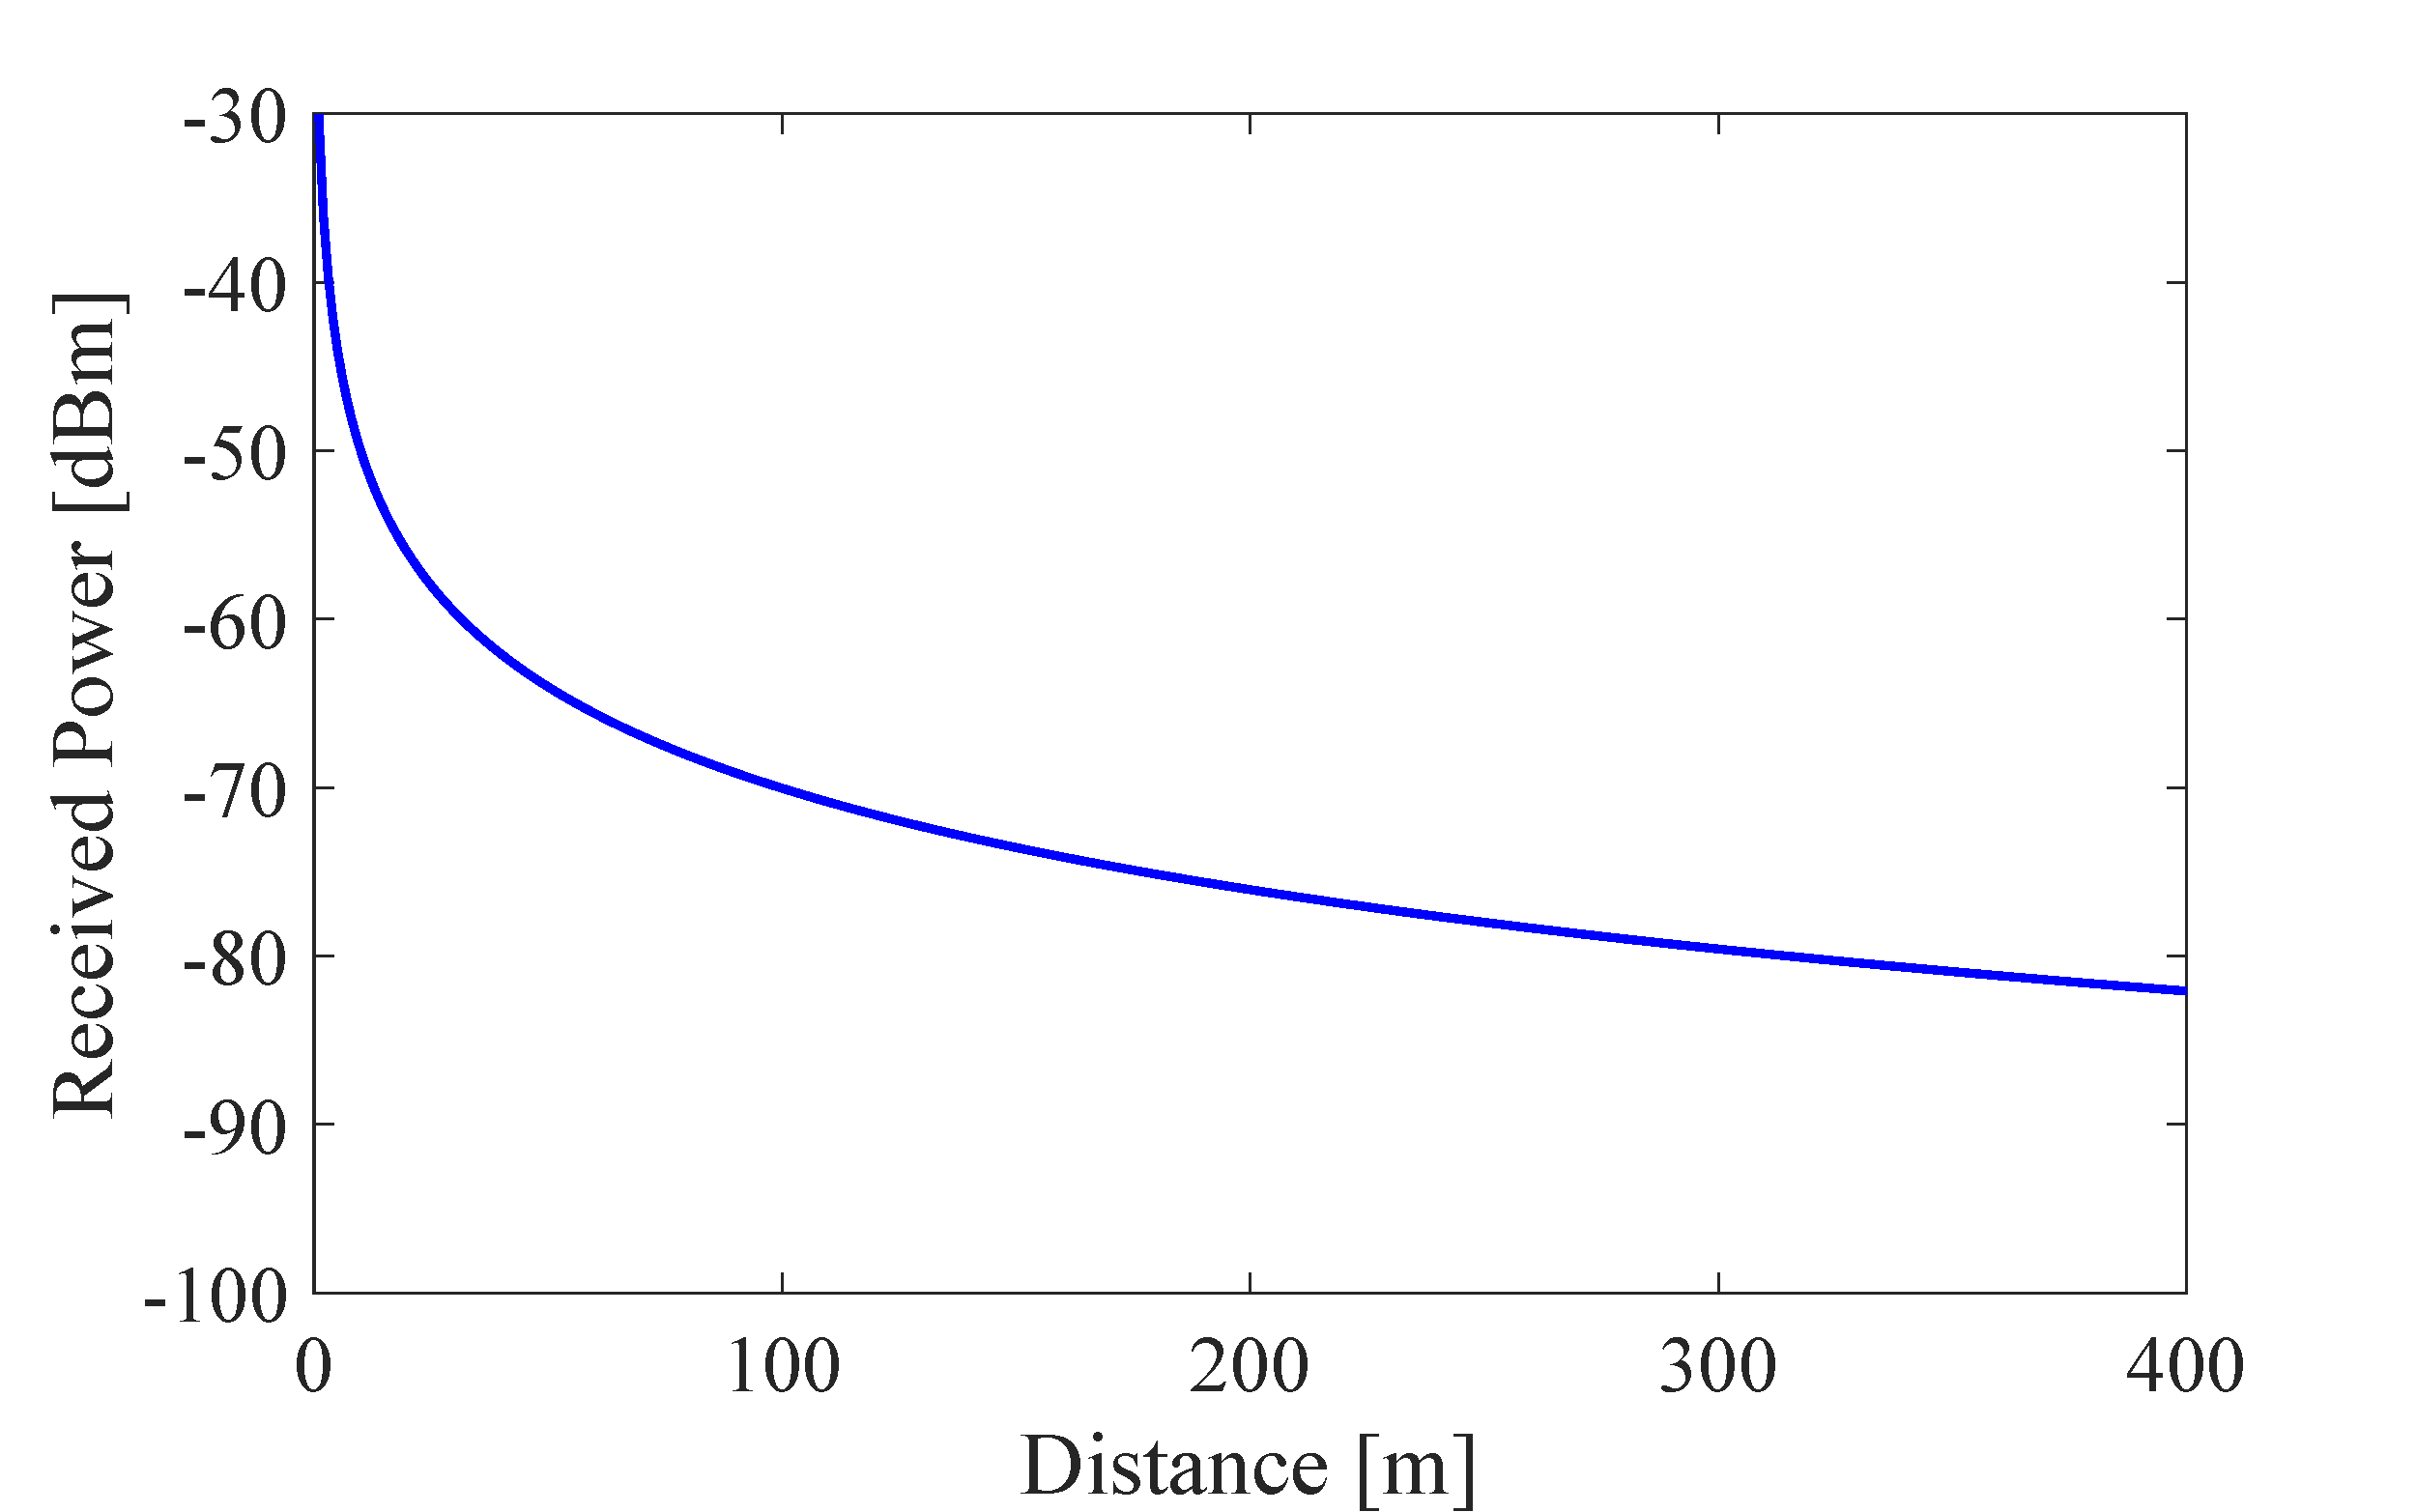
\includegraphics[width=\linewidth]{lfsp_vs_distance.pdf} % 図のファイル名を指定
  \caption{送受信局間の距離に対する受信電力}
  \label{fig:Received power_vs_distance} % 参照用ラベル
\end{figure}


\begin{figure}[H]
  \centering
  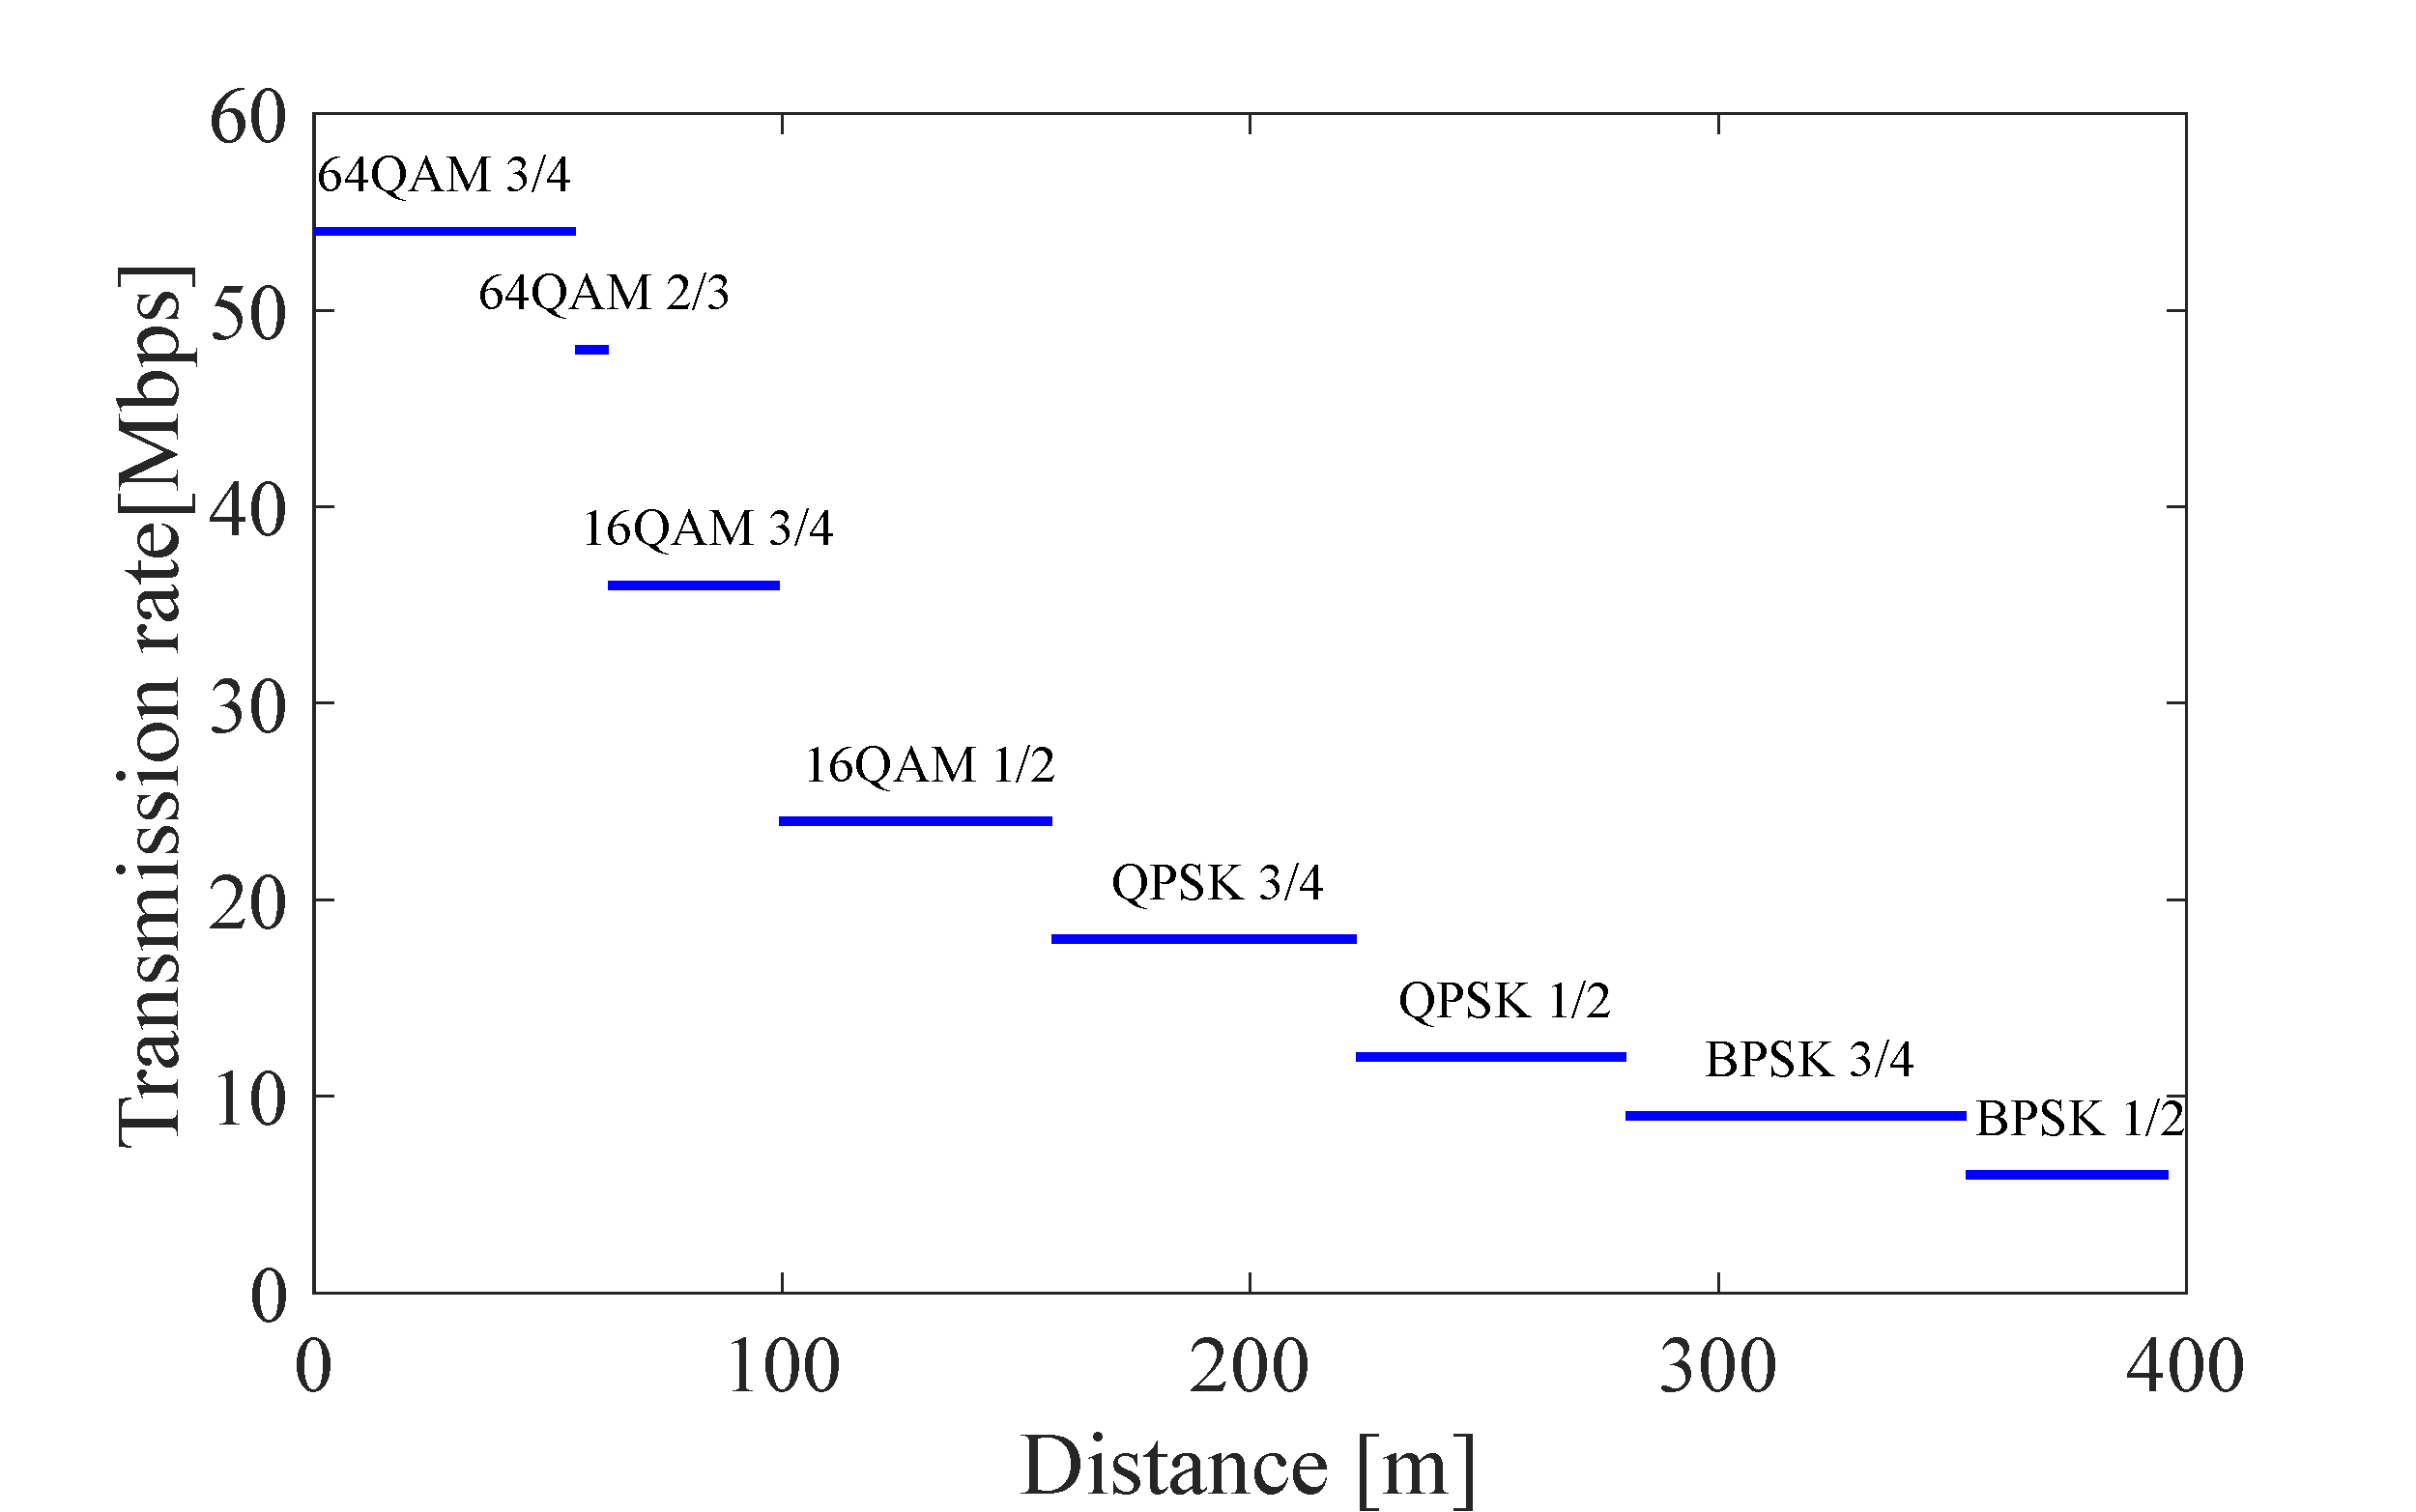
\includegraphics[width=\linewidth]{rate_vs_distance.pdf} % 図のファイル名を指定
  \caption{伝送レートと距離の関係}
  \label{fig:rate_vs_distance} % 参照用ラベル
\end{figure}

\begin{figure}[H]
  \centering
  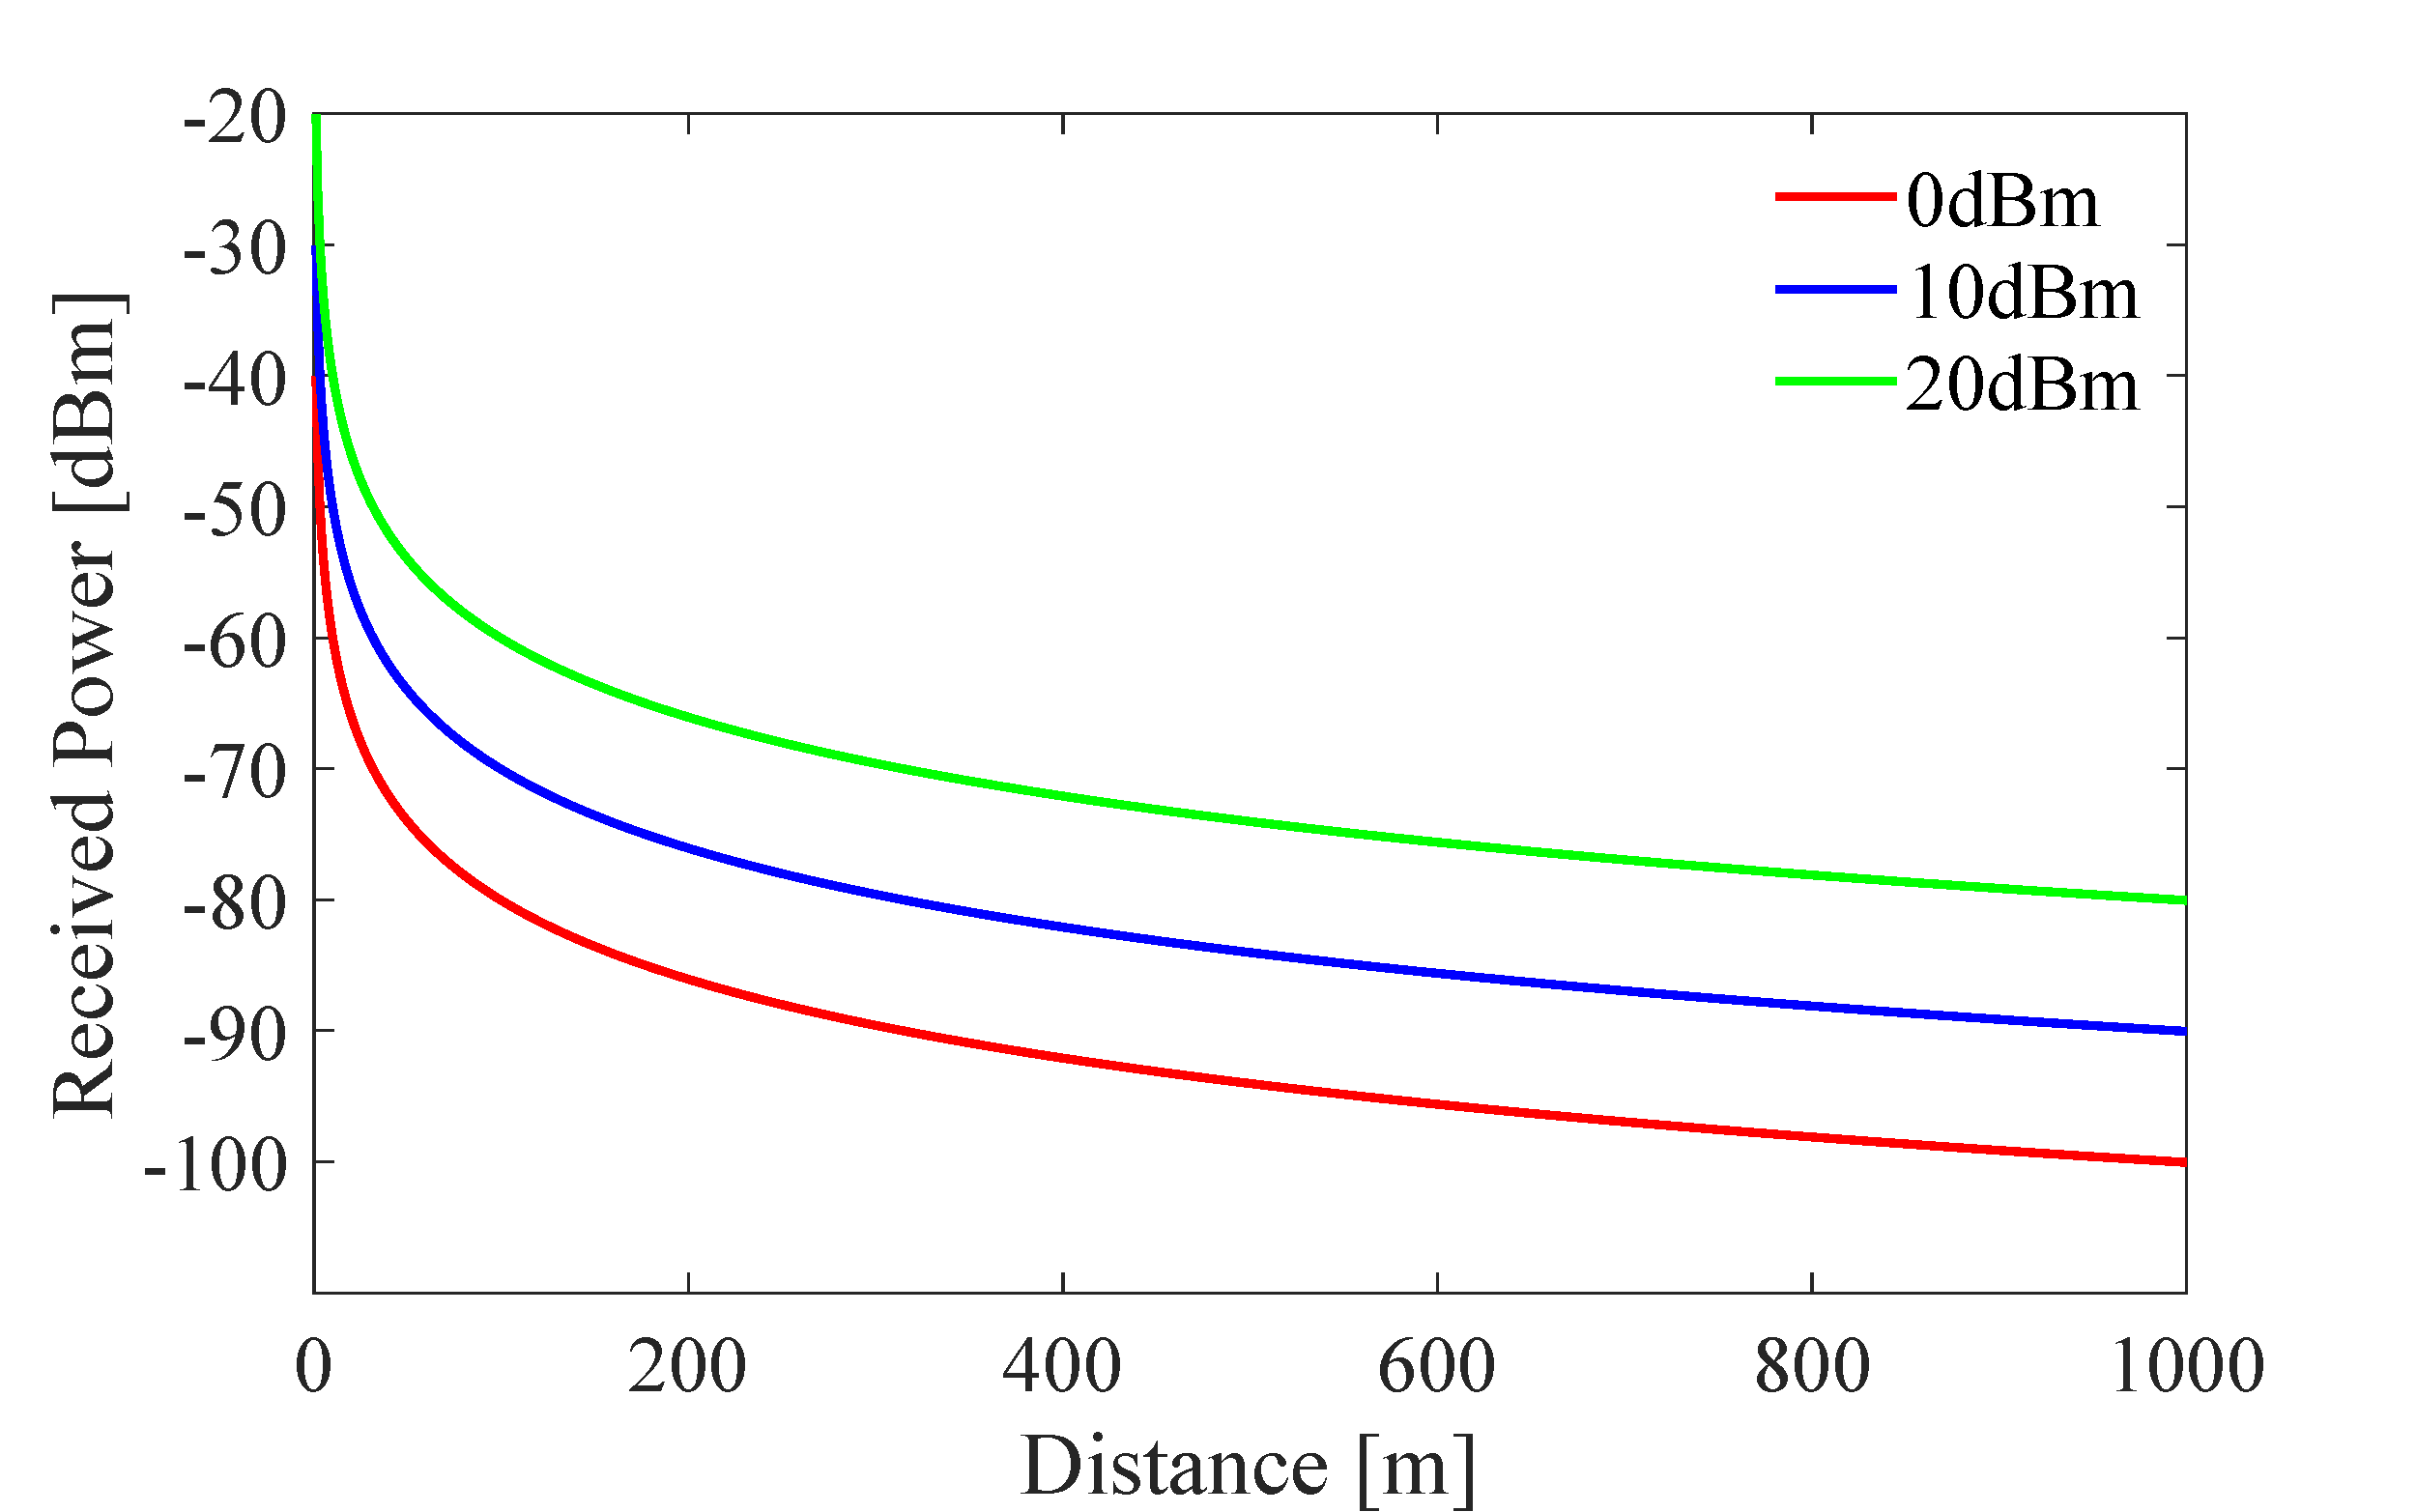
\includegraphics[width=\linewidth]{lfsp_vs_distance_2.pdf} % 図のファイル名を指定
  \caption{各送信電力の送受信距離に対する受信電力}
  \label{fig:lfsp_vs_distance_2} % 参照用ラベル
\end{figure}

\begin{figure}[H]
  \centering
  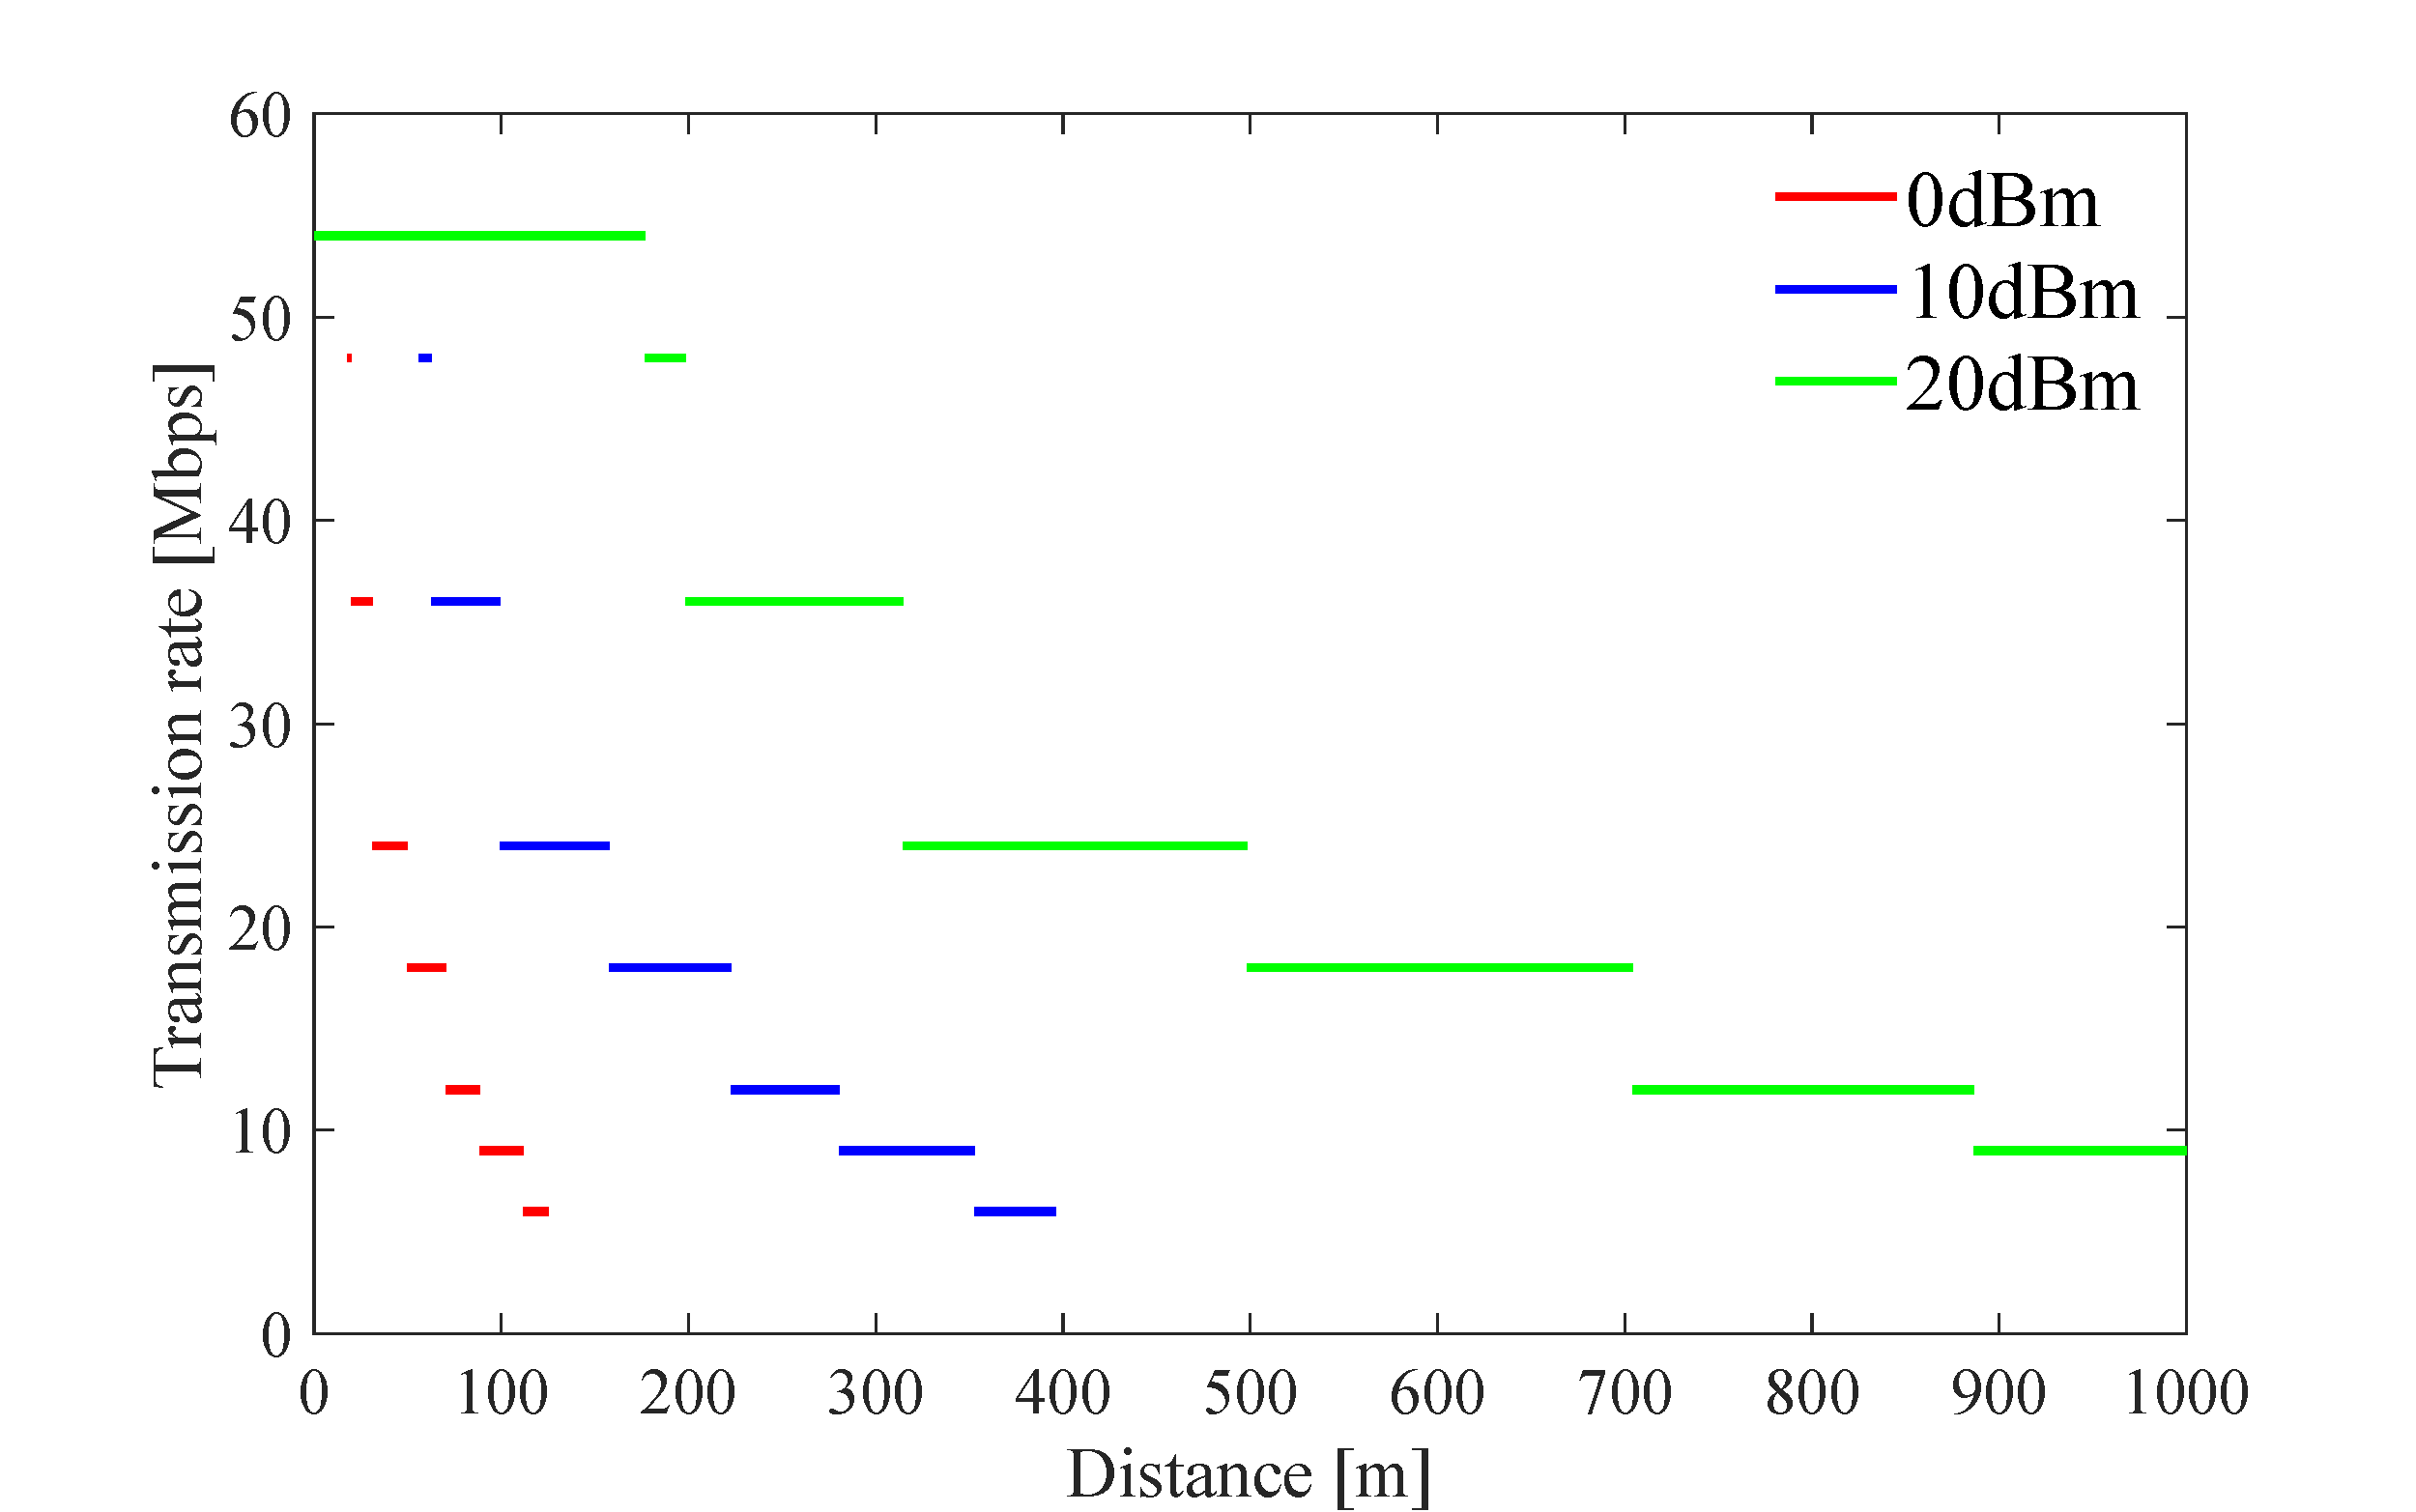
\includegraphics[width=\linewidth]{rate_vs_distance_2.pdf} % 図のファイル名を指定
  \caption{各伝送レートと距離の関係}
  \label{fig:rate_vs_distance_2} % 参照用ラベル
\end{figure}

\clearpage
\subsection{CSMA/CA方式}
本節では同一無線チャネルを複数の無線局で共有して通信するためのアクセス制御方式であるCSMA/CA(Carrnse Multiier Seple Access with Collision Avoidance)方式及びそれを用いた2進数バックオフ制御とDCF(Distributed Coordination Funciton)方式について説明する.\par
図\ref{fig:CSMA/CA}にCSMA/CA方式のアクセス制御を示す.
無線通信では,複数の端末が共通の通信チャネルを利用するため,同時にフレームを送信すると衝突が発生し,通信の品質が低下する可能性がある.
CSMA/CA方式は,キャリアセンスによってデータを送信する前にチャネルが空いている(Idle)かどうかを判断する.
チャネルが空いている場合に,ランダムなバックオフ時間を設けて,バックオフ時間待った後再度キャリアセンスを行い,チャネルがIdleであればフレーム送信を試みる手法である.
受信局はフレームを正常に受信した場合,ACK(Acknowledgement)フレームを送信する.送信局はACKフレームを受信することでフレーム送信が成功したと判断し,ACKを受信できなかった場合,衝突が発生したとみなして再送を行う.
無線通信では,CSMA/CD(Carrier Sense Multiple Access with Collision Detection)方式のような衝突検出が困難なため,事前に衝突を回避するためのランダムバックオフが採用されている.
IEE802.11規格では,2進数バックオフが標準規格で定義されている.\par
\begin{figure}[H]
  \centering
  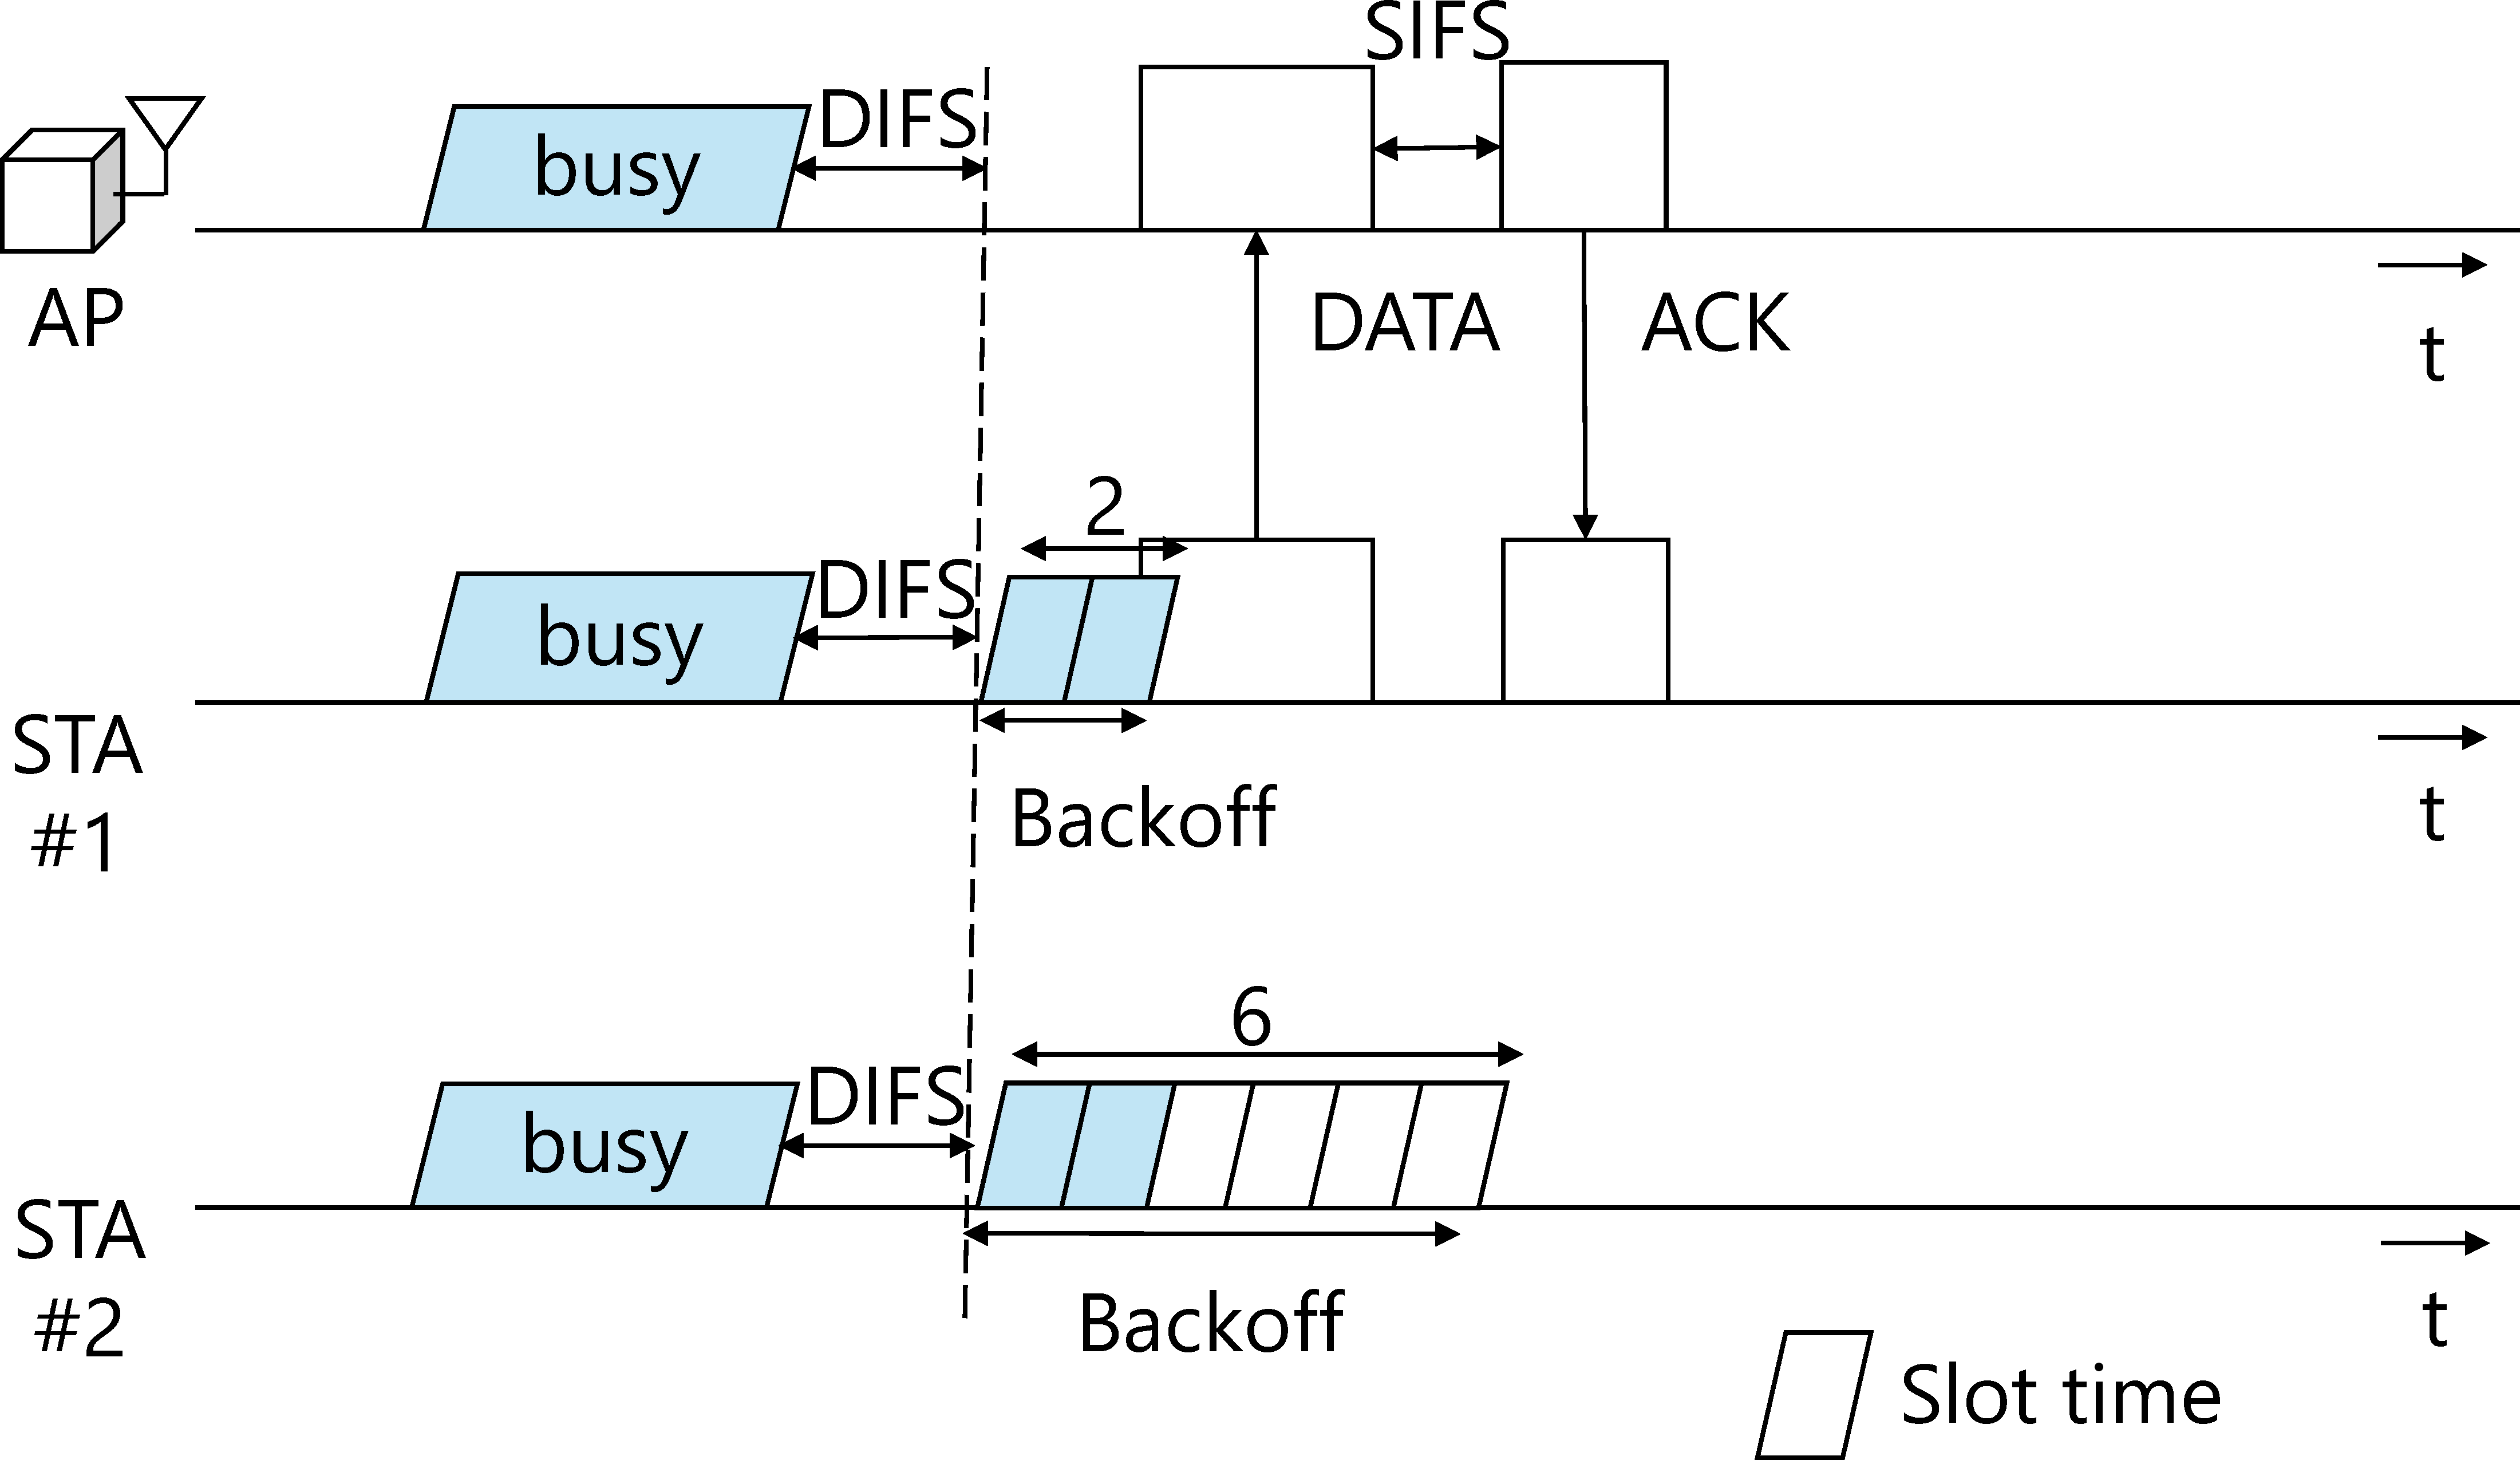
\includegraphics[width=\linewidth]{CSMACA.pdf} % 図のファイル名を指定
  \caption{CSMA/CA方式のアクセス制御}
  \label{fig:CSMA/CA} % 参照用ラベル
\end{figure}

2進数バックオフ制御では,ランダムなバックオフ時間を設定し,バックオフ時間が経過した送信局が送信権を獲得する.
このランダムな待ち時間(バックオフ時間)はCW(Contenion Window)と呼ばれる[0,$CW$]の範囲の一様乱数を発生させ,その乱数値をもとに決められる.
バックオフ時間は一定時間(スロット・タイム)の倍数であり,チャネルがIdleであればバックオフ時間をスロット・タイムごとに減算していき,最後に0となった無線局が送信を行う.
衝突によって再送を試みる度に$CW$の範囲は最大サイズ($CW_{\text{max}}$)まで2倍ずつ増加し,フレーム送信が成功した場合は$CW$の範囲は範囲が最小値($CW_{\text{min}}$)に縮小される.
バックオフ時間は,
\begin{equation}
 \text{Backoff}  = \text{Random()} \times \text{Slottime}
\end{equation}
と表され,Random()(乱数値)は[0,$CW$]の範囲の一様乱数である.
また,$CW$の範囲は次式で表される.
\begin{equation}
  CW_n = 2^{n} \times (CW_{\text{min}}+1)-1
  \label{eq:CW}
\end{equation}
ここで,$n$は再送回数を表し,$CW_n$は再送回数が$n$のときの$CW$の範囲である.
IEEE802.11gでは,$CW_{\text{min}}$は15,$CW_{\text{max}}$は1023となっている.
再送を繰り返し,$CW_{\text{max}}$に達したときはあらかじめパラメータで決められた最大再送回数M回となるまでは$CW$の範囲は変えずに$CW_{\text{max}}$ままとしM回再送に失敗したフレームは破棄される.
また,バックオフアルゴリズムでは$CW$の範囲により衝突確率と送信時間のトレードオフとなっている.
つまり,$CW$の範囲が小さいと送信までに要する時間は短いが,衝突確率が高くなり,$CW$が大きいと送信までに要する時間が長くなるが衝突確率が低くなる.\par
次にDCF方式について説明する.IEEE802.11規格では2進数バックオフCSMA/CAをベースにフレーム間隔のIFS(InterFrame Space)や再送制御機能を加えたDCF方式が採用されている.
IEEE802.11規格には,IFSは信号を送信する前に最低限の送出信号間隔として定義されている.IFSの長さは6種類存在し,DIFS(Distributed Inter Frame Space)やSIFS(Short Inter Frame Space) が代表的である.
これらは,優先順位に基づいて異なるIFSが選択される.
具体的には,最も優先順位の高く,フレーム間隔が短いのがSIFSで,DIFSはSIFSよりも長く,優先順位が低い.
DCFで用いられる通常のデータ・フレームは,優先度の低いフレーム間隔であるDIFSを使用し,応答についてはデータ・フレームを受け取り次第,送信側に正常に受信したことを知らせるACKフレームを最優先のSIFS時間を用いて送信する.\par
図\ref{fig:DCF}にDCF方式の概要を示す.
DCFはチャネルがDIFS期間でBusyの場合,送信局はランダムなバックオフ時間の後にフレームを送信する.
バックオフ時間においてチャネルがIdleになったスロット時間ごとに、バックオフ値を1ずつ減らし,バックオフ値が0になると送信権を獲得しフレームを送信する.
このとき,送信フレームを持つ他無線局は図\ref{fig:DCF}(b) に示すように現在のバックオフ値を次回の送信時に持ち越す.
例えば図\ref{fig:DCF}(b)では,STA\#2と\#3の$CW$サイズは5であり,STA\#1の$CW$サイズの2よりも待ち時間が長いため,STA\#1が最初に送信権を獲得し,STA\#2とSTA\#3は残ったバックオフ値3を次回のバックオフに持ち越す.
フレームを送信した送信局は宛先受信局からの確認応答(ACK)フレームの応答が無い場合,フレーム送信が成功しなかった
と判断して式\ref{eq:CW}にしたがって$CW$の範囲を2倍にして再送信する.この手順はフレームが正常に送信されるか,送信がキャンセルされるまで実行される.

\begin{figure}[p]
  \centering
  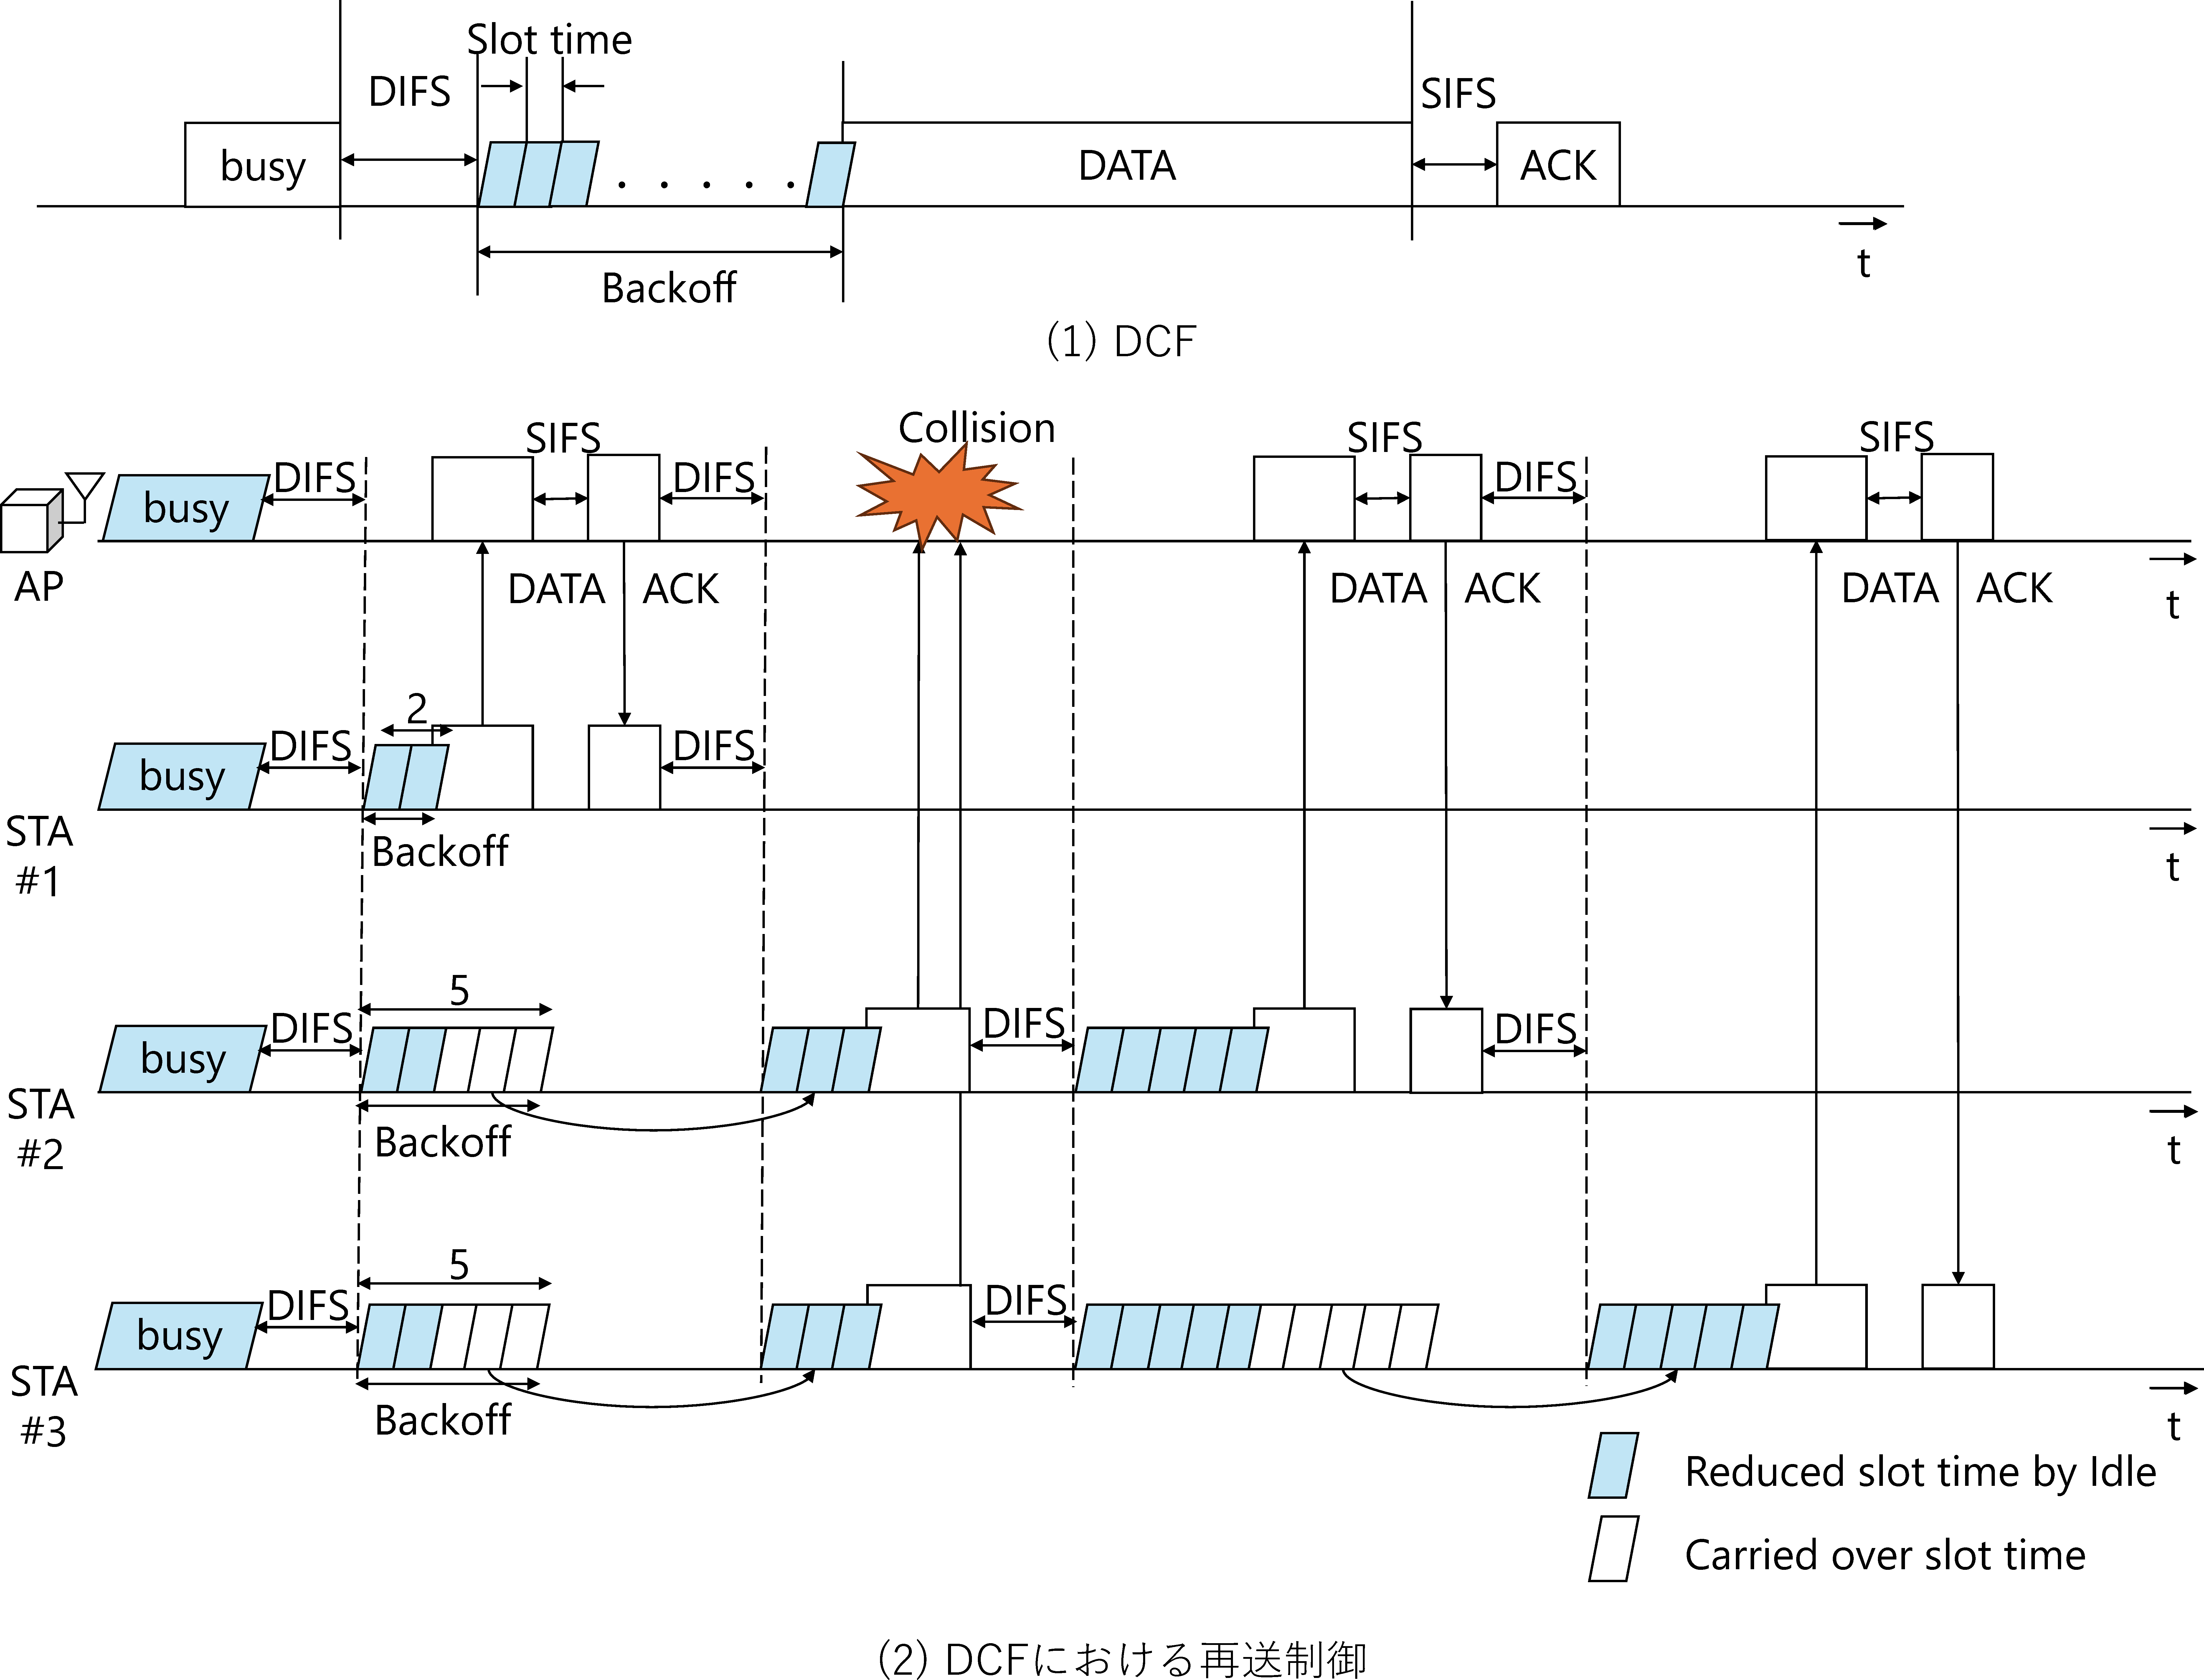
\includegraphics[width=\linewidth]{DCF.pdf} % 図のファイル名を指定
  \caption{DCF制御}
  \label{fig:DCF} % 参照用ラベル
\end{figure}
\clearpage
\subsection{IEEE802.11gのスループット}
本節ではIEEE802.11gのスループット(単位時間当たりのデータ転送量)の計算手法について説明する.
ここでは1対1のユニキャスト通信,誤りやパケットの衝突による再送は無いと仮定してDCFにおけるスループットを計算する.
図\ref{fig:11g_packet}に802.11gのDCFを用いたIPレベルのスループットの計算モデルを示す.
IPレベルのパケット長を最大の1500byteとするとIPレベルのスループット=1500byte/Tとなる.
802.11ACKが返された後に続くデータ・パケットは,DCFのバックオフ制御に基づいて送信される.
誤りやパケットの衝突による再送は無いと仮定すると,DCFのバックオフ制御の平均時間は

\begin{equation}
   DIFS+\frac{CW_{min}}{2} \times \text{Slottime}
\end{equation}
となる.ここで$CW_{\text{min}}$は$CW$(乱数の発生範囲)の最小値である.\par
図\ref{fig:11g_frameformat}に802.11gのフレームフォーマットと計算式を示す.
802.11gのOFDM変調を用いる場合には,PLCPフレームの長さはOFDMシンボル4$\mu$sの整数倍となるようにパディング・ビット(調整用に付加するフレーム)により調整され,802.11gの場合のみ6$\mu$sの無信号期間が付加される.
また802.11gでは,802.11bとの互換性を重視する場合には長さが20$\mu$sのスロット・タイムを使用するが,802.11aと同様のスループットが得られるショート・スロット・タイム(9$\mu$s)も定義されている.
図\ref{fig:11g_throughput}に802.11gのショート・スロット・タイム使用時のIPレベルのスループットの計算結果を示す.
伝送レートが大きくなるにつれてスループットが上昇することが確認できるが,物理レイヤとMACレイヤのオーバーヘッドの影響が大きくなり効率が低下することが確認できる.


\begin{figure}[H]
  \centering
  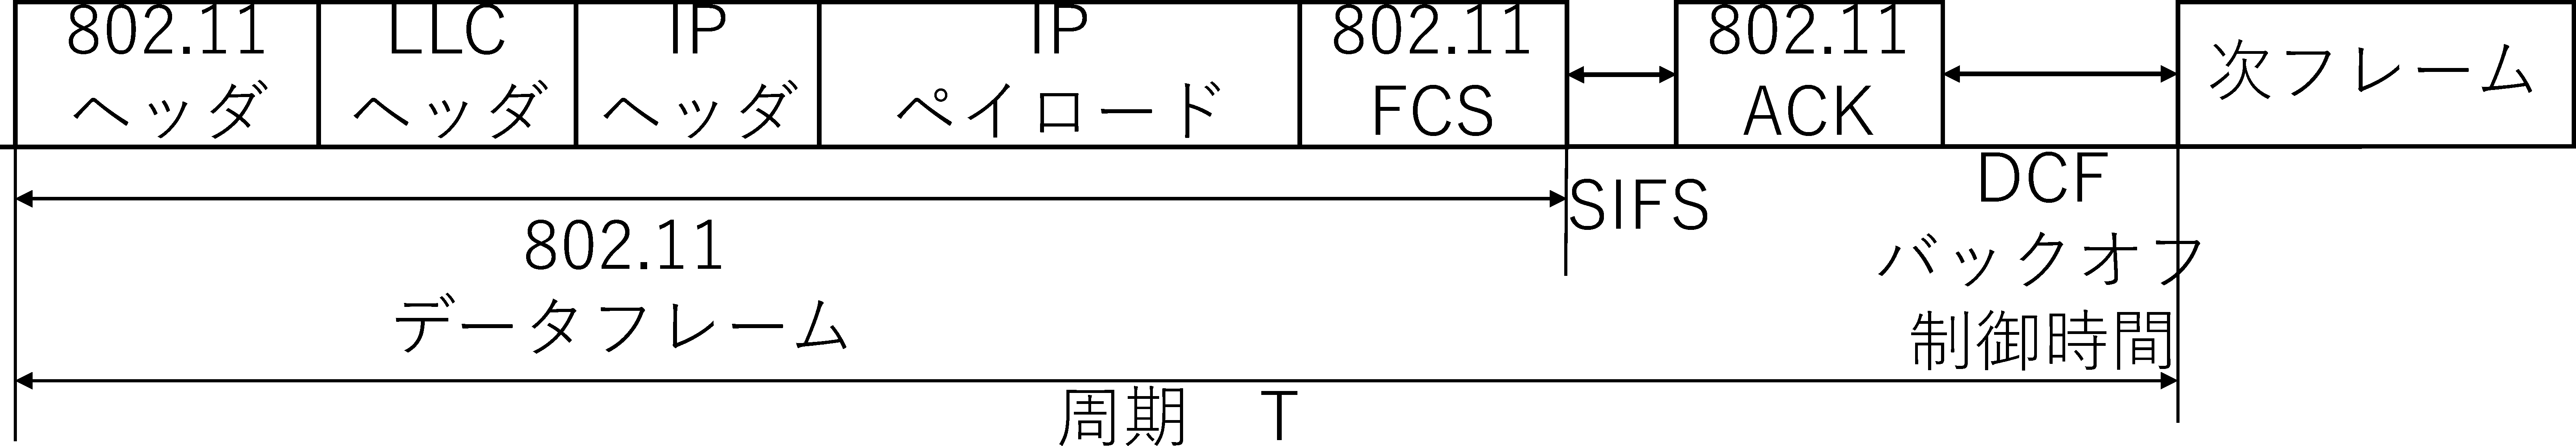
\includegraphics[width=\linewidth]{11g_packet.pdf} % 図のファイル名を指定
  \caption{IPレベルのスループットの計算モデル}
  \label{fig:11g_packet} % 参照用ラベル
\end{figure}

\clearpage
\begin{figure}[p]
  \centering
  \includegraphics[width=\linewidth]{11g_frameformat.pdf} % 図のファイル名を指定
  \caption{IEEE802.11gの計算式}
  \label{fig:11g_frameformat} % 参照用ラベル
\end{figure}
\clearpage
\begin{figure}[H]
  \centering
  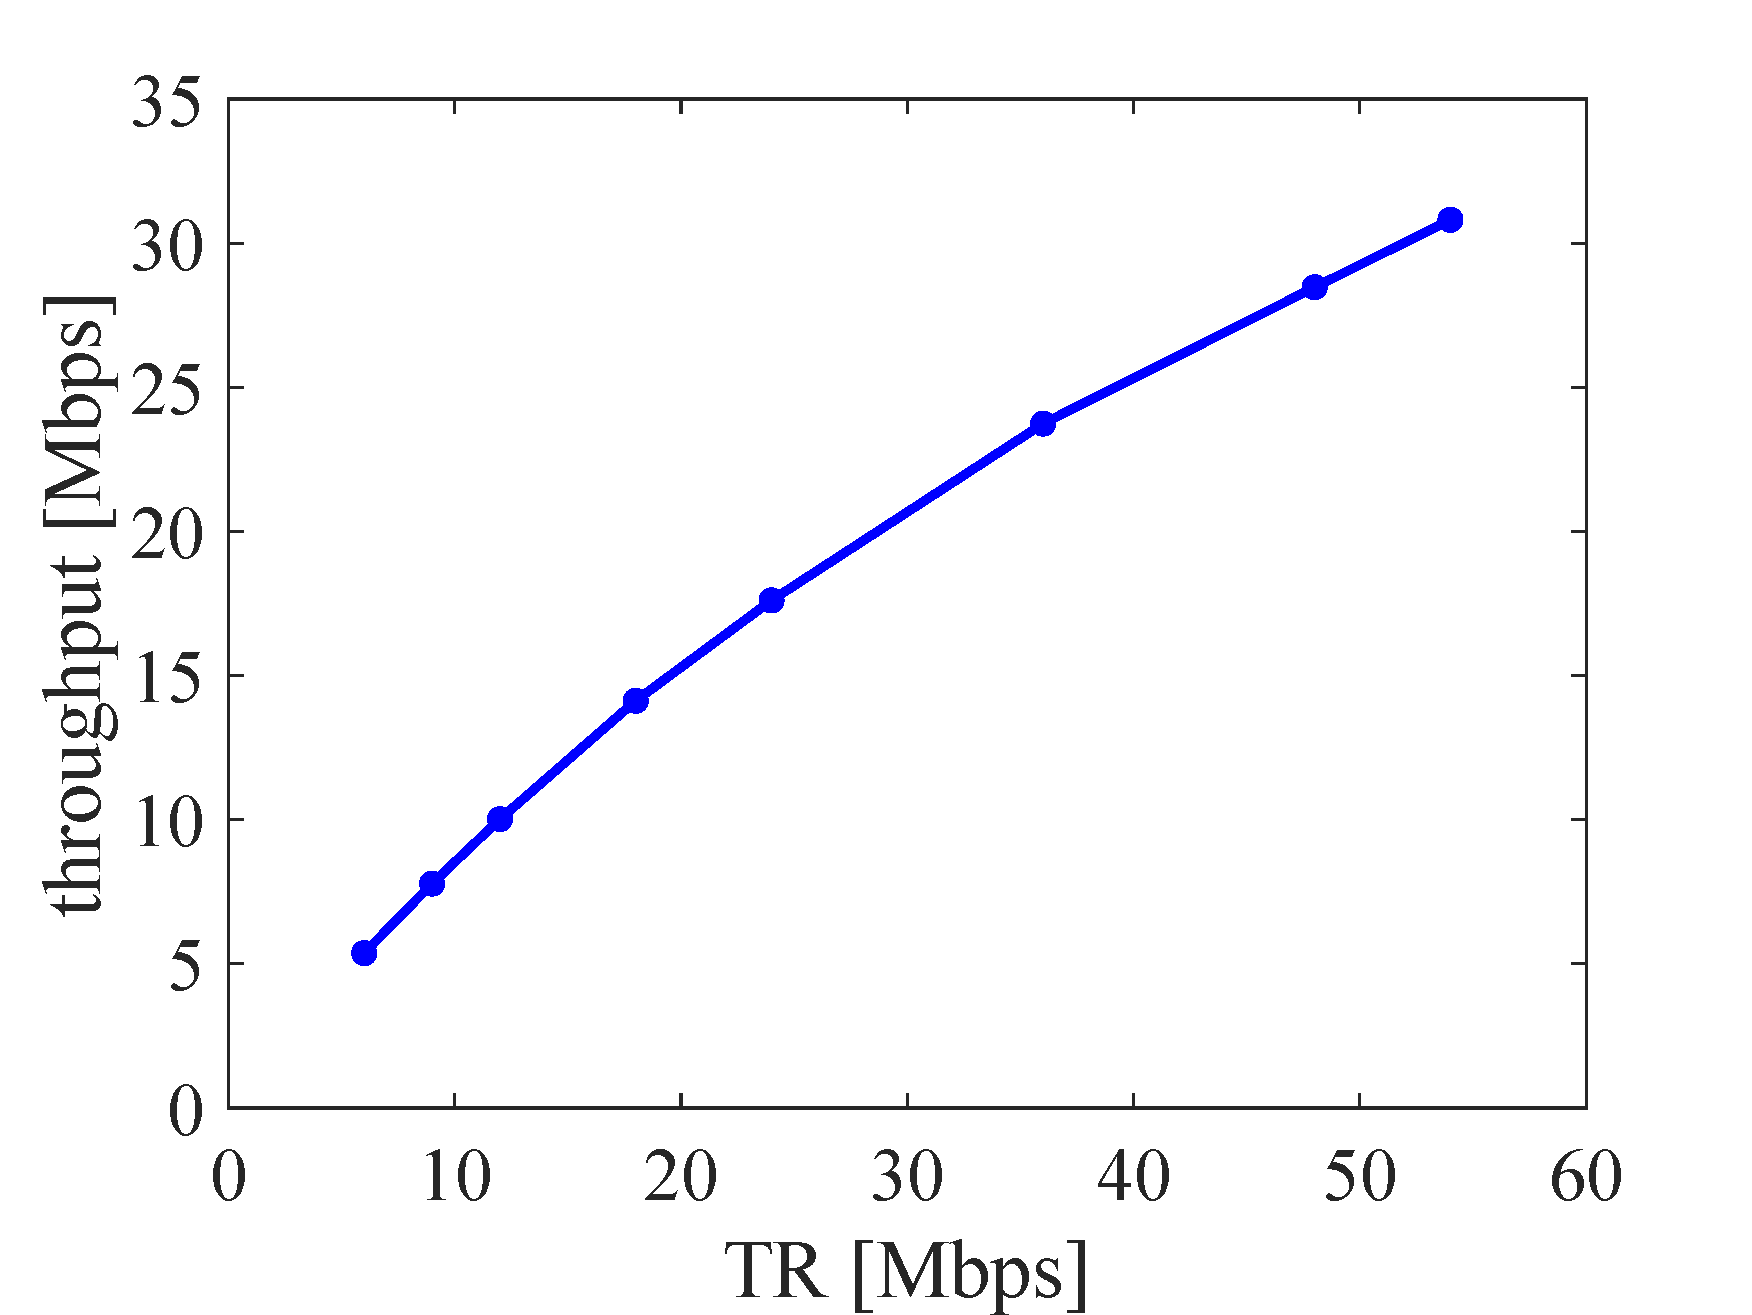
\includegraphics[width=\linewidth]{g_throughput.pdf} % 図のファイル名を指定
  \caption{ショート・スロット・タイム使用時のIPレベルのスループット}
  \label{fig:11g_throughput} % 参照用ラベル
\end{figure}


% ******************************************************
% 3.従来方式の概要
% ******************************************************
\clearpage
\section{従来方式の概要}

従来の中継伝送方式では指向性アンテナ/ビームを利用した1ホップずつの中継伝送となっている.
自由空間では,電力の伝搬損失が自遊空間伝搬損失なので地上通信と比べて伝搬損失が小さい.
また,指向性アンテナ/ビームを用いる場合,無指向性アンテナと比べて送受信のアンテナ利得が大きくなる.
したがって,送信信号が中継先のドローンよりも遠方のドローンに到達するためオーバーリーチ干渉が発生する.\par
図\ref{fig:conventional_topology}に従来方式である概要を示す.
図のように送信信号が中継先のドローン(図1\#3)より遠くのドローン(図1\#4)に到達することで干渉が生じる.
図\ref{fig:lfsp_vs_distance_3}に自由空間伝搬損失(伝搬乗数=2)と地上屋外伝搬(伝搬乗数=2.6)の距離に対する受信電力特性を示す.
アンテナ利得は2.14dBi,送信電力は10dBmで,式\ref{eq:friis},\ref{eq:lfsp}に基づいて計算した.
無線LANなどの最低受信感度は約-90dBmなので,地上屋外伝搬では約100 m程の伝送距離となる.
一方,で自由空間伝搬では約1000mまで送信信号が届き,非常に遠方でも送信信号が減衰しない.
このことから,直線の中継伝送ではオーバリーチ干渉の影響が大きくなるため解決方法の検討が必要となる.
また,従来方式で干渉が生じ,再送を行う際には,フォールバック制御により伝送レートを下げることでSNRが低くてもフレームを受信できるようにしている.
そのため,伝送レートの低下に伴って送信時間や再送によるオーバヘッドが増加して効率が低下する問題もある.


\begin{figure}[H]
  \centering
  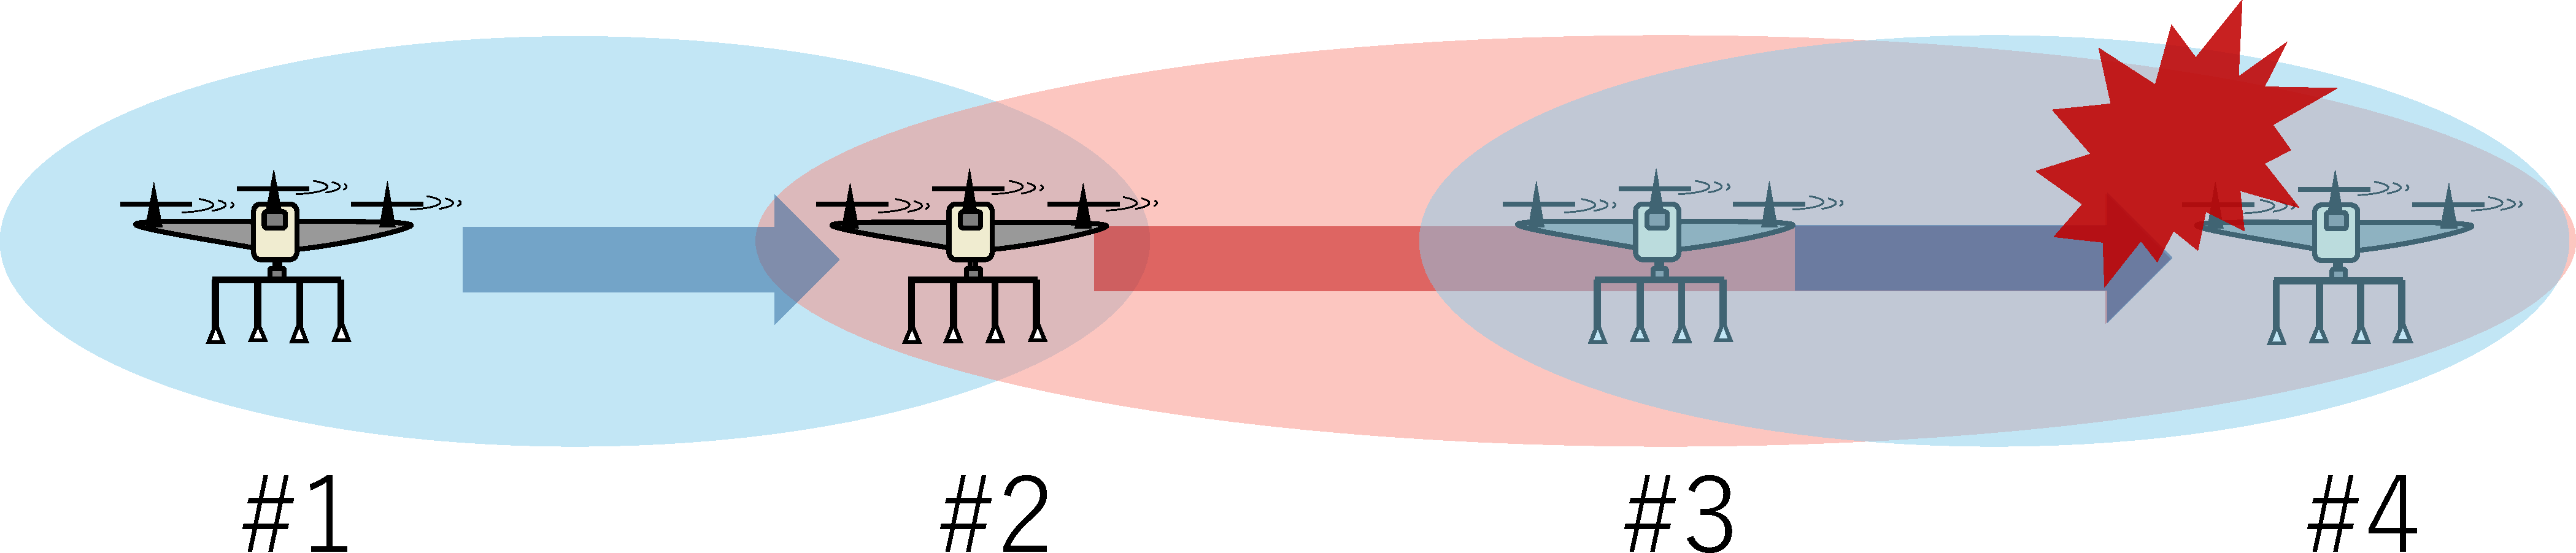
\includegraphics[width=\linewidth]{cenventional_topology.pdf} % 図のファイル名を指定
  \caption{従来の方式の概要}
  \label{fig:conventional_topology} % 参照用ラベル
\end{figure}

\begin{figure}[H]
  \centering
  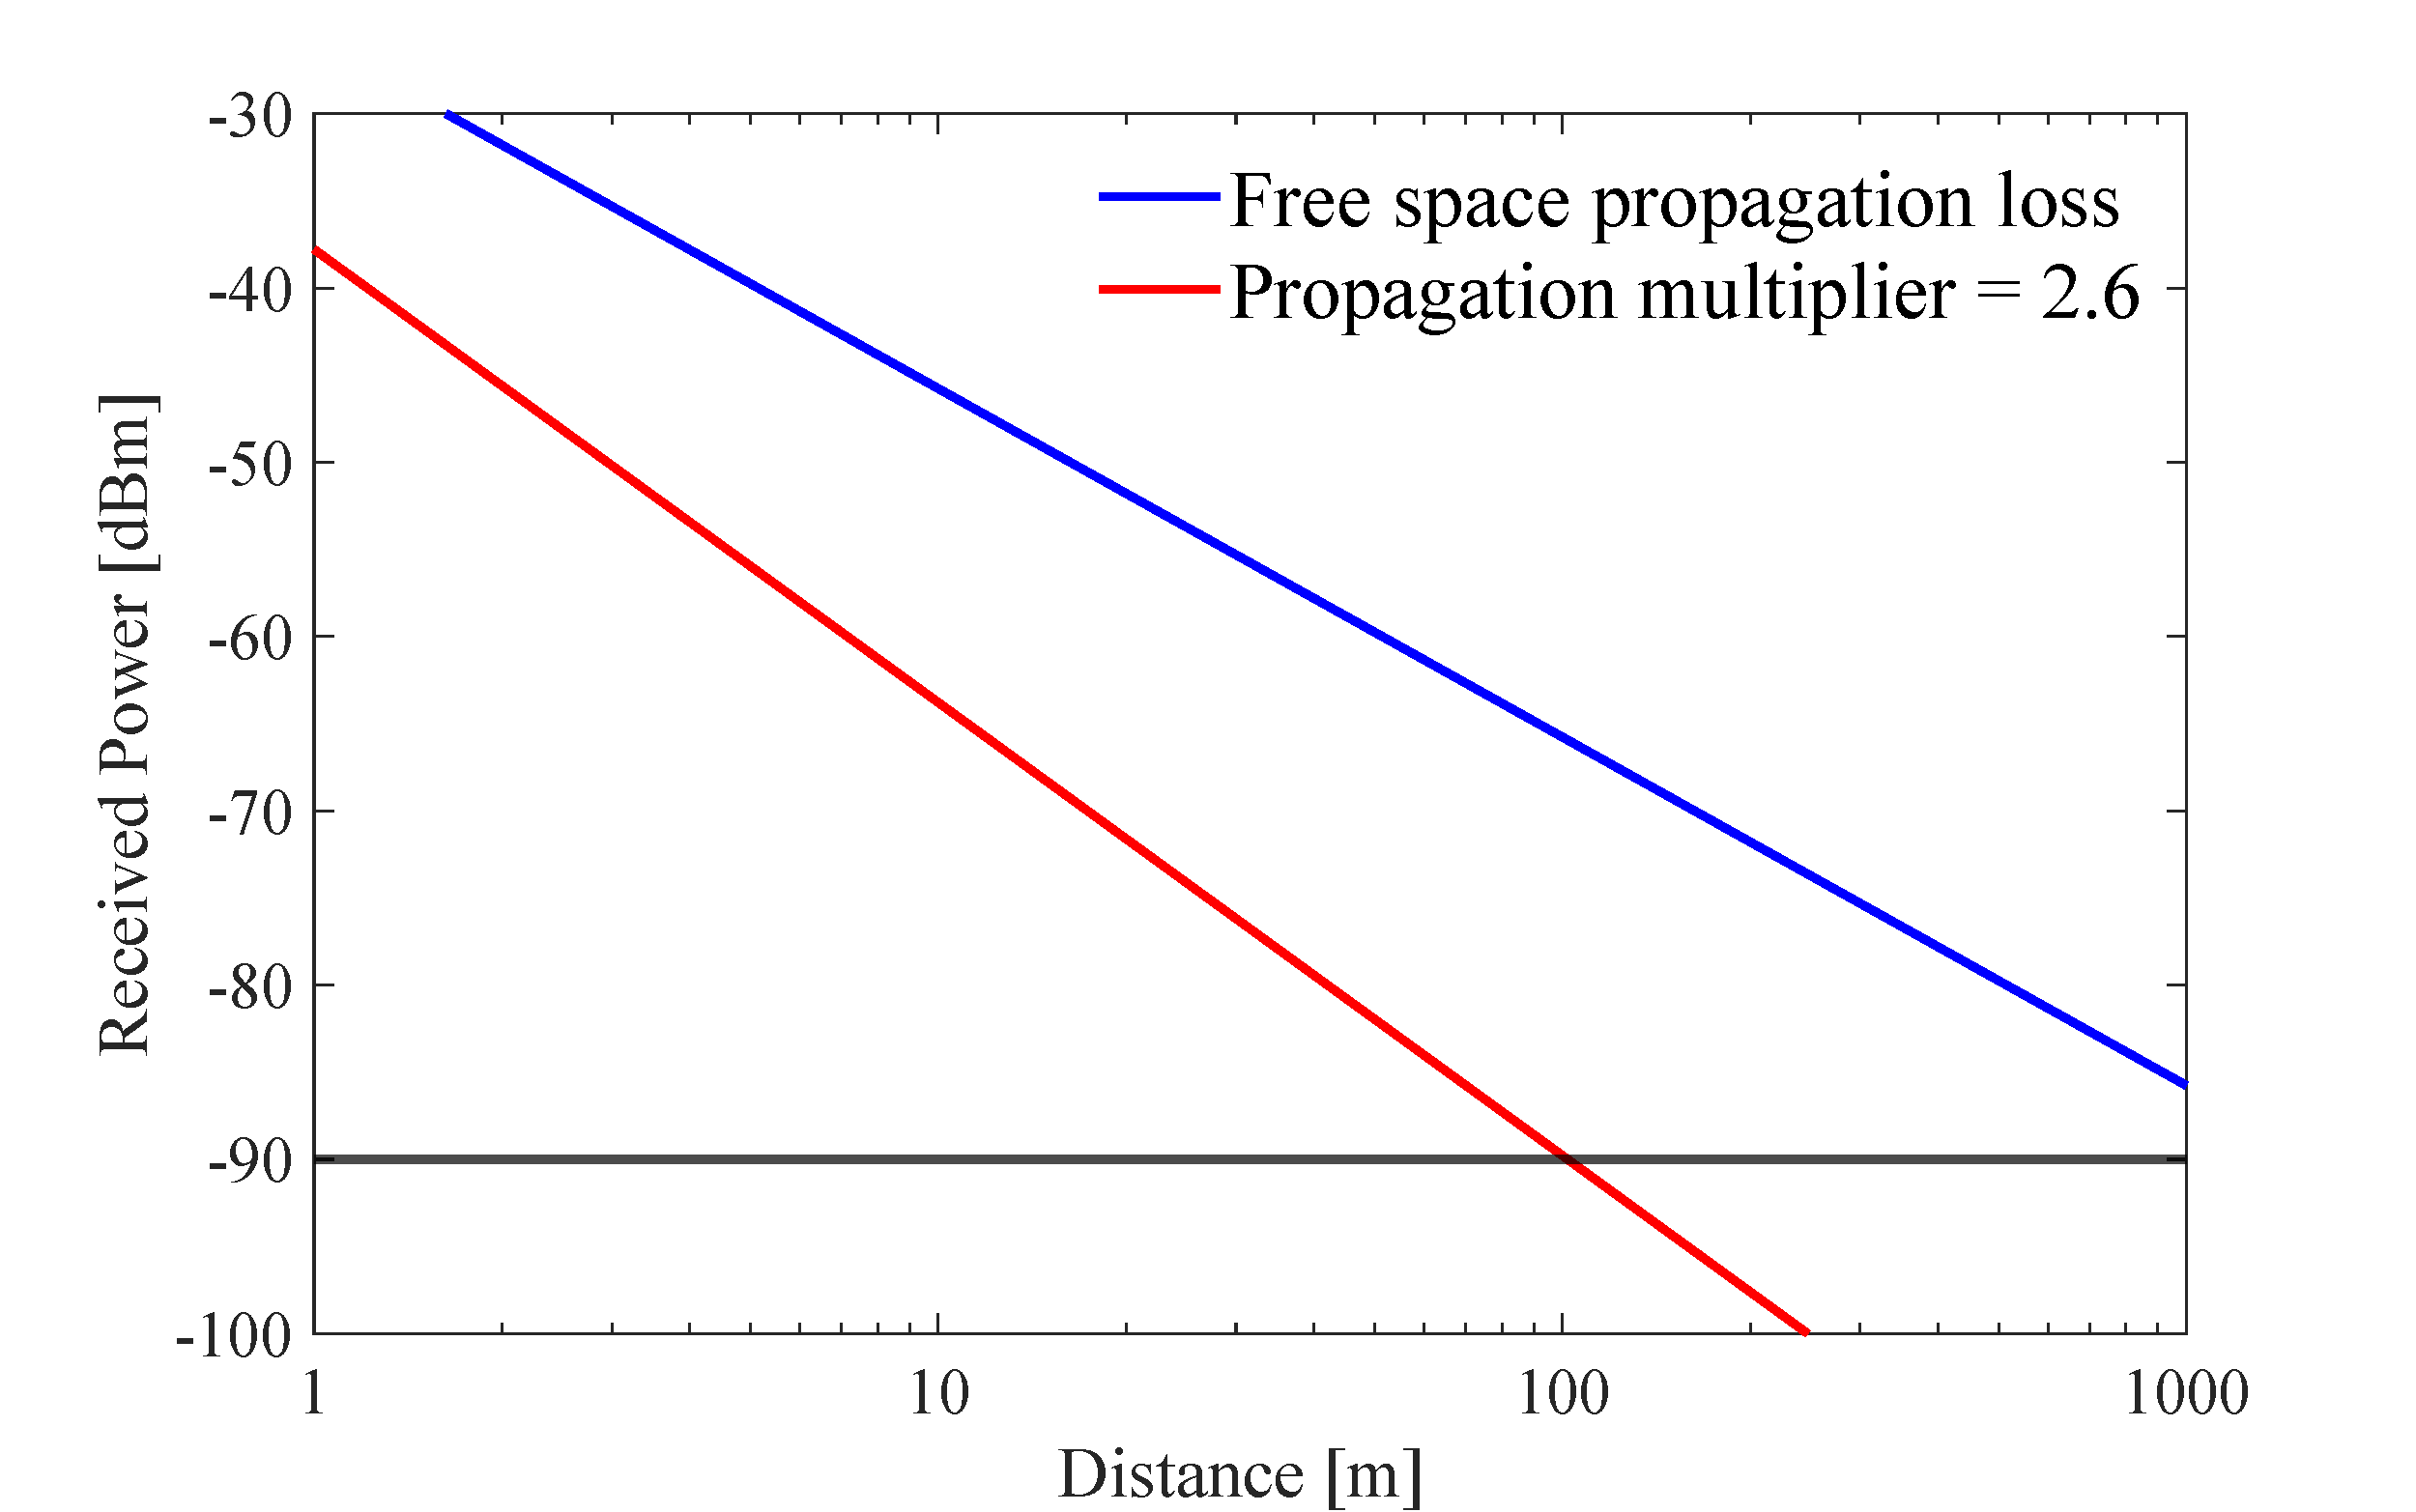
\includegraphics[width=\linewidth]{lfsp_vs_distance_3.pdf} % 図のファイル名を指定
  \caption{距離に対する受信電力特性}
  \label{fig:lfsp_vs_distance_3} % 参照用ラベル
\end{figure}

% ******************************************************
% 4.CTR方式の概要
% ******************************************************
\clearpage
\section{CTR方式の概要}

オーバリーチ干渉は送信信号が中継局のドローンを超えて他のドローンに干渉することで発生する.そこでCTR方式では直線状に存在する中継局が協調することによってオーバリーチ干渉の問題を解決する.
図\ref{fig:CTR_topology}に示すCTR方式は,送信信号の届く範囲の最終中継局(図\ref{fig:CTR_topology}\#4)まで一度に信号を送信し,通信経路の中継局(図\ref{fig:CTR_topology}\#3)も協調してパケットを受信する.
最終中継局がパケットを正常に受信した場合は,以後,同様の手順で中継する.
最終中継局がパケットの受信に失敗した場合は,直線経路の中継局\#3が\#4の代わりに次の中継局へパケットを中継する.
そのため従来方式ではオーバーリーチ干渉が生じる環境でもCTR方式ではオーバーリーチ干渉が減り中継ホップ数も減るので中継オーバヘッドも削減することができる.

\begin{figure}[H]
  \centering
  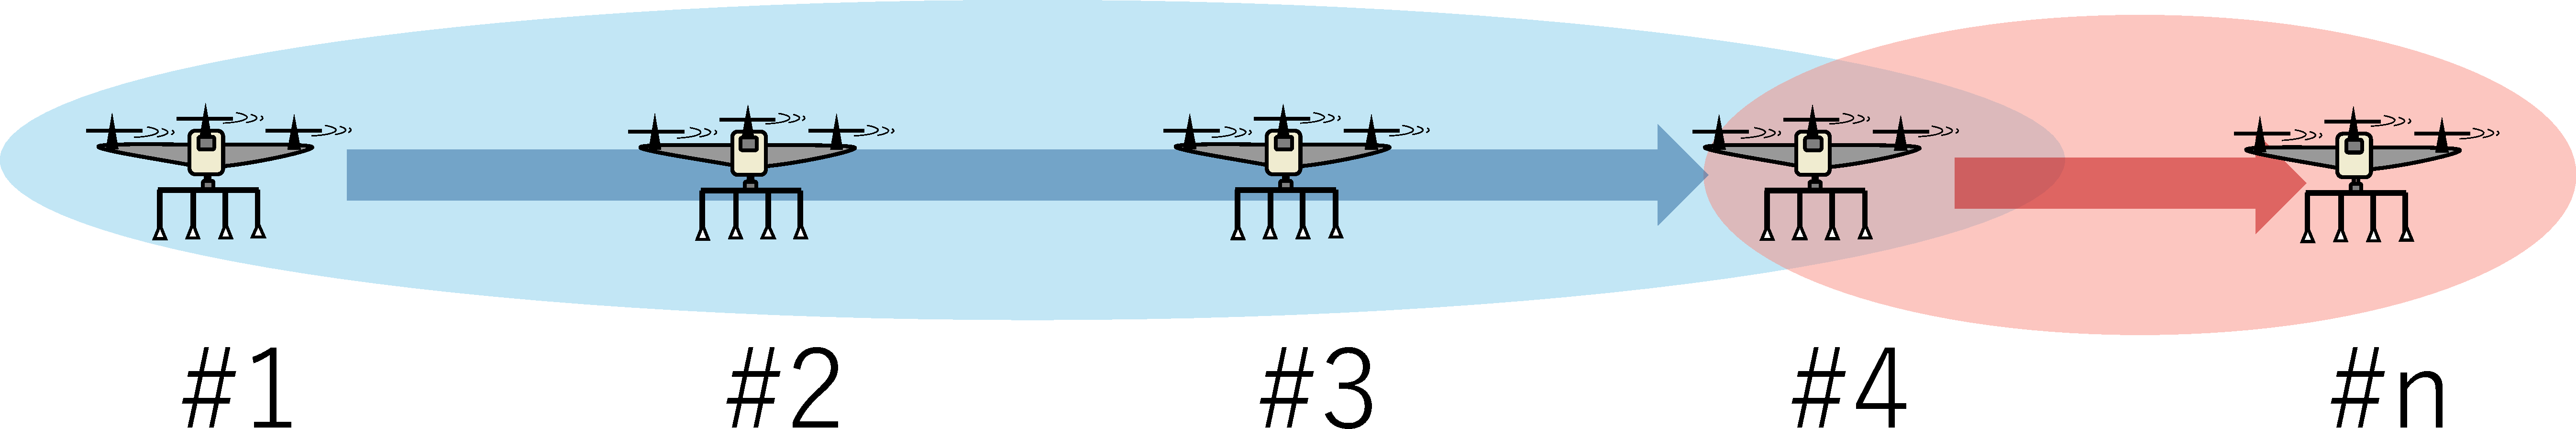
\includegraphics[width=\linewidth]{CTR_topology.pdf} % 図のファイル名を指定
  \caption{CTR方式の概要}
  \label{fig:CTR_topology} % 参照用ラベル
\end{figure}

図\ref{fig:CTR_accsess}にCTR方式の詳細なアクセス制御手順を示す.
本方式では,最終中継局がパケットを受信できなかった場合でも中継を継続できる仕組みが導入されている.
送信局がランダムなバックオフ時間の後,ACK durationを記述したパケットを送信する.
パケットを受信した中継局は,指定されたACK duration後に送信局へACKを返信する.ACK durationはスロットタイムで区切られ,最終受信中継局が最短のACK durationを持ち,送信局に近づくにつれてスロットタイムが1ずつ増加する設計となっている.
これは送信電力の制御や,各端末のSNRおよび受信電力閾値に基づく自律的な判断を行い信号が到達する最大範囲を推定することでスロットタイムが適切に設定される仕組みとなっている.
具体的には,図\ref{fig:CTR_accsess}\#4がパケットを受信した場合,スロットタイムは受信電力より\#3,\#2の順番で増加し,送信局の\#1にACKを返信すると,経路上の中継局である\#2,\#3はACKの送信待ちをキャンセルする.
最終受信中継局(図\ref{fig:CTR_accsess}\#4)がパケットの受信に失敗した場合は\#3が送信局の\#1にACKを送信し,\#4の代わりとして中継を続行する.
これにより,従来方式の再送でのオーバーヘッドの増加や,フォールバック制御による伝送レートの低下を防ぐことができる.
\begin{figure}[H]
  \centering
  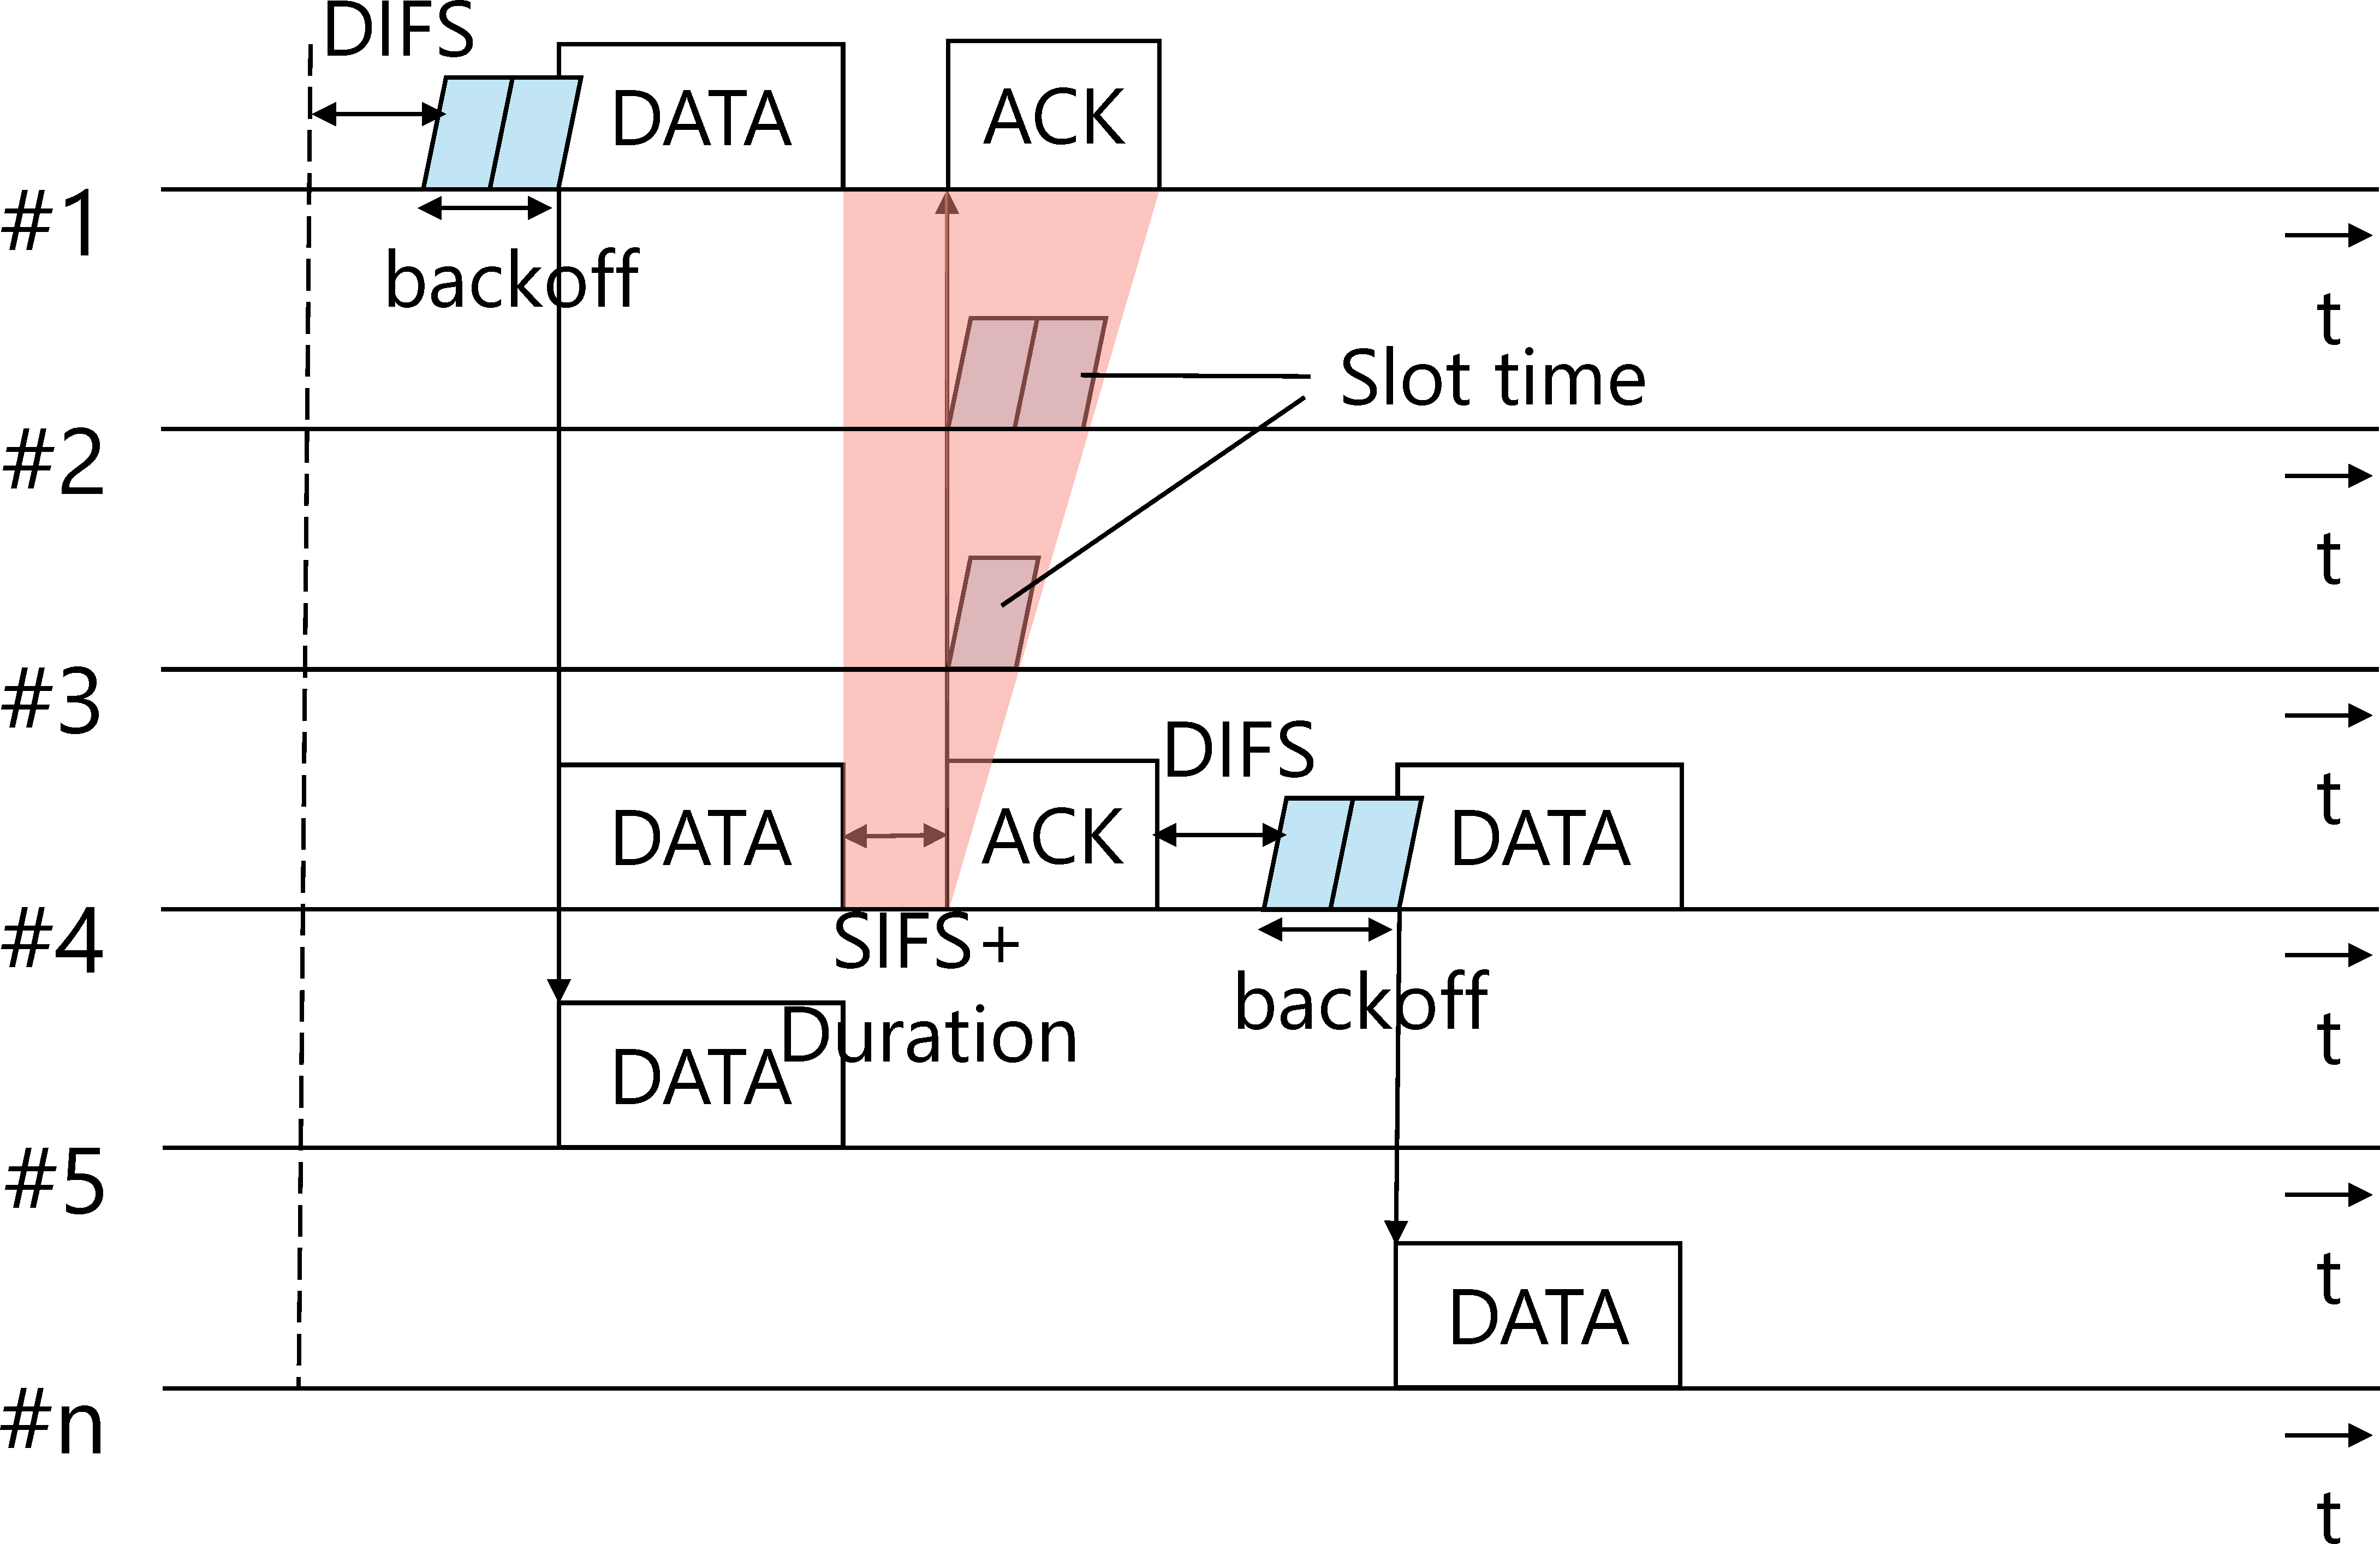
\includegraphics[width=\linewidth]{CTR_accsess.pdf} % 図のファイル名を指定
  \caption{CTR方式のアクセス制御}
  \label{fig:CTR_accsess} % 参照用ラベル
\end{figure}

% ******************************************************
% 5.従来方式とCTR方式の評価と比較
% ******************************************************
\clearpage
\section{従来方式とCTR方式の評価と比較}
\subsection{誤りが無い条件でのCTR方式の評価}
CTR方式の特徴である中継局をスルーすることによるスループットの向上を以下の条件で従来方式と比較する.
図\ref{fig:CTR_model}にドローンのトポロジーを示す.
中継の総伝送距離は1000mとし,50m間隔で直線状に20台のドローンを配置した.アンテナの送受信利得は0dBi,送信電力は10dBmとした.周波数は2.4GHz,伝送レートはIEEE 802.11gを参考にし,伝搬損失は自由空間伝搬損失とした.
評価内容は従来の1ホップ中継(54Mbps) と中継局を2台スルー(24Mbps) した場合,および中継局を3台スルー(18Mbps) した場合におけるスループット特性を確認する.
括弧内は使用可能な最も高い伝送レートである.
これは受信電力より,2章の表\ref{tab:IEEE802.11g_TR&Modulation}に基づいて決定した.
また,1000mを伝送するのにかかった時間に対する各伝送レートごとのオーバヘッドとペイロードの送信時間を確認する.

図\ref{fig:throughput_through} にCTR方式と従来方式のスループット特性を示す.従来の1ホップ中継と比べてCTR方式で中継局を3台スルーした条件では約2倍のスループットが得られた.
図\ref{fig:overhead_vs_paylord}に各伝送レートにおけるオーバヘッドとペイロードの送信時間を示す.
ペイロードの部分は中継回数に応じて分割している.
伝送レートが低いほどオーバヘッドが減少し,従来の1ホップ中継CTR方式の3台スルーした条件では約1/4に減少することが確認できる.
また,ペイロードの一回の送信時間は伝送レートが高いほど短くなるが,中継回数が増加するため総合した送信時間は短くならない.
そのため,ドローンをスルーする場合は,通信距離が長くなり使用可能な伝送レートが低下するが、アクセス制御やプリアンブル等のオーバヘッドとのトレードオフになり,その結果,ネットワーク全体の通信効率において,中継局を3台スルーする条件が最も高くなることを確認した.


\begin{figure}[H]
  \centering
  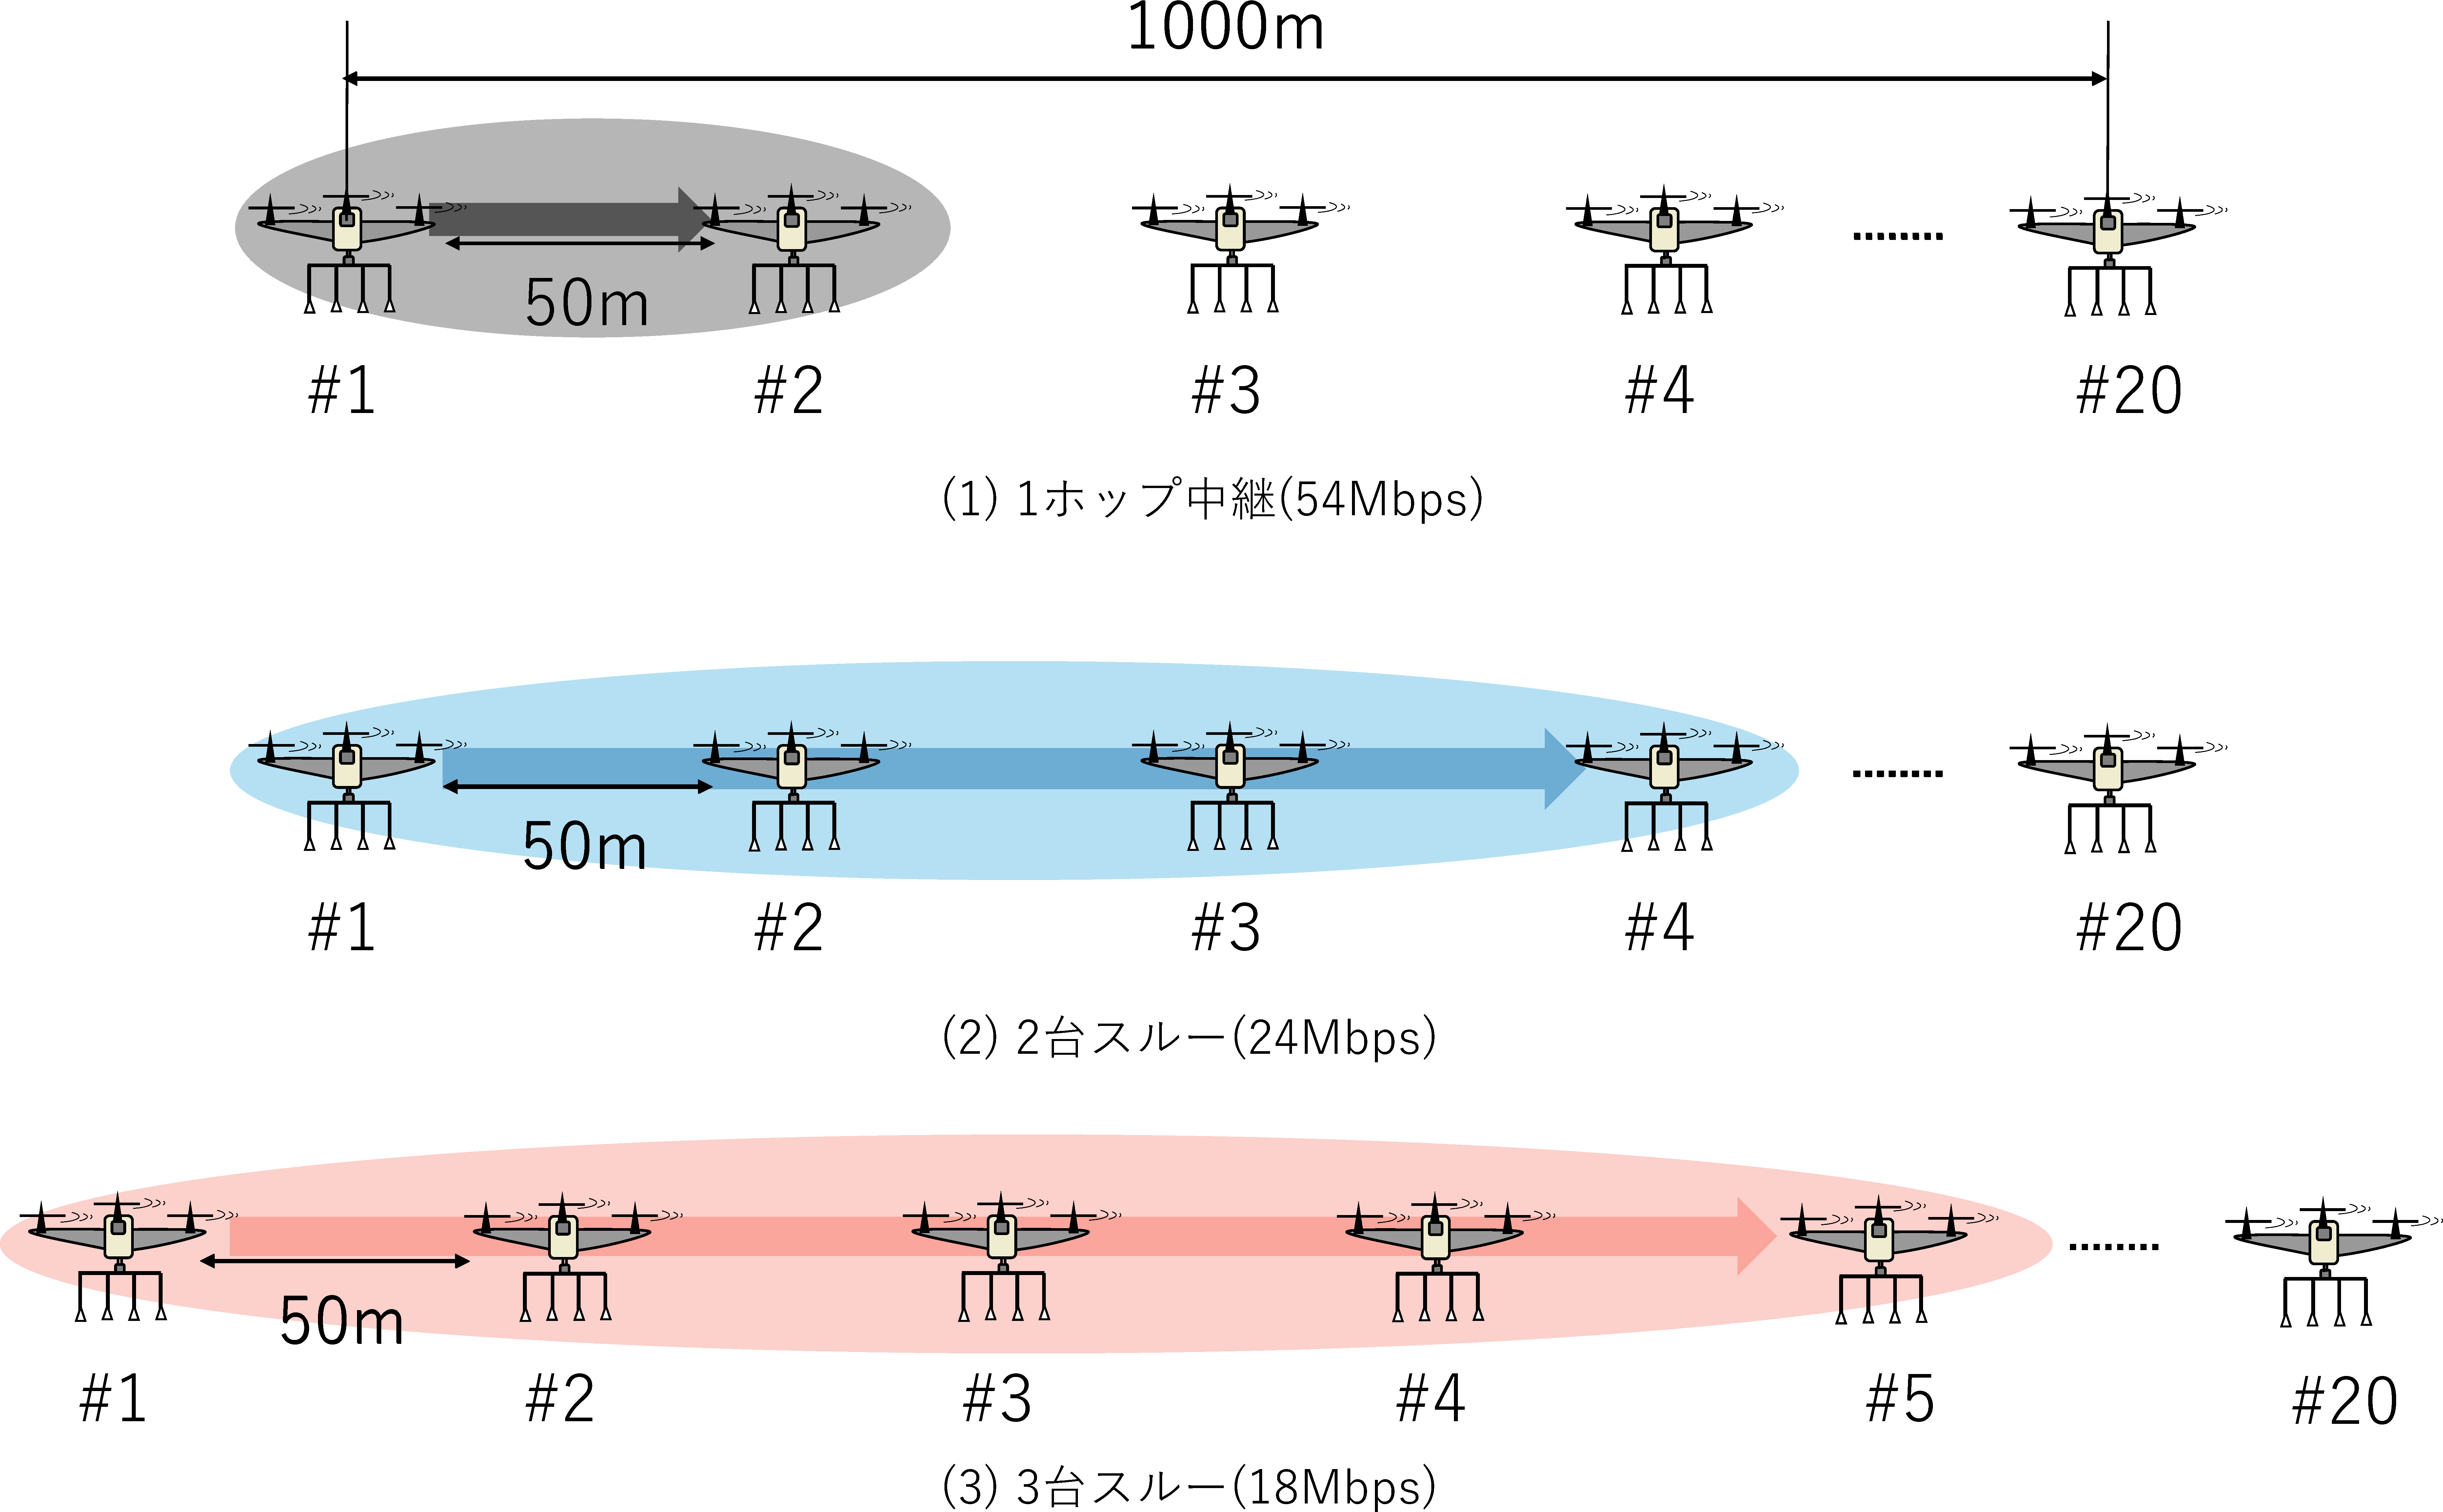
\includegraphics[width=\linewidth]{CTR_model.pdf} % 図のファイル名を指定
  \caption{従来方式とCTR方式のトポロジー}
  \label{fig:CTR_model} % 参照用ラベル
\end{figure}

\begin{figure}[H]
  \centering
  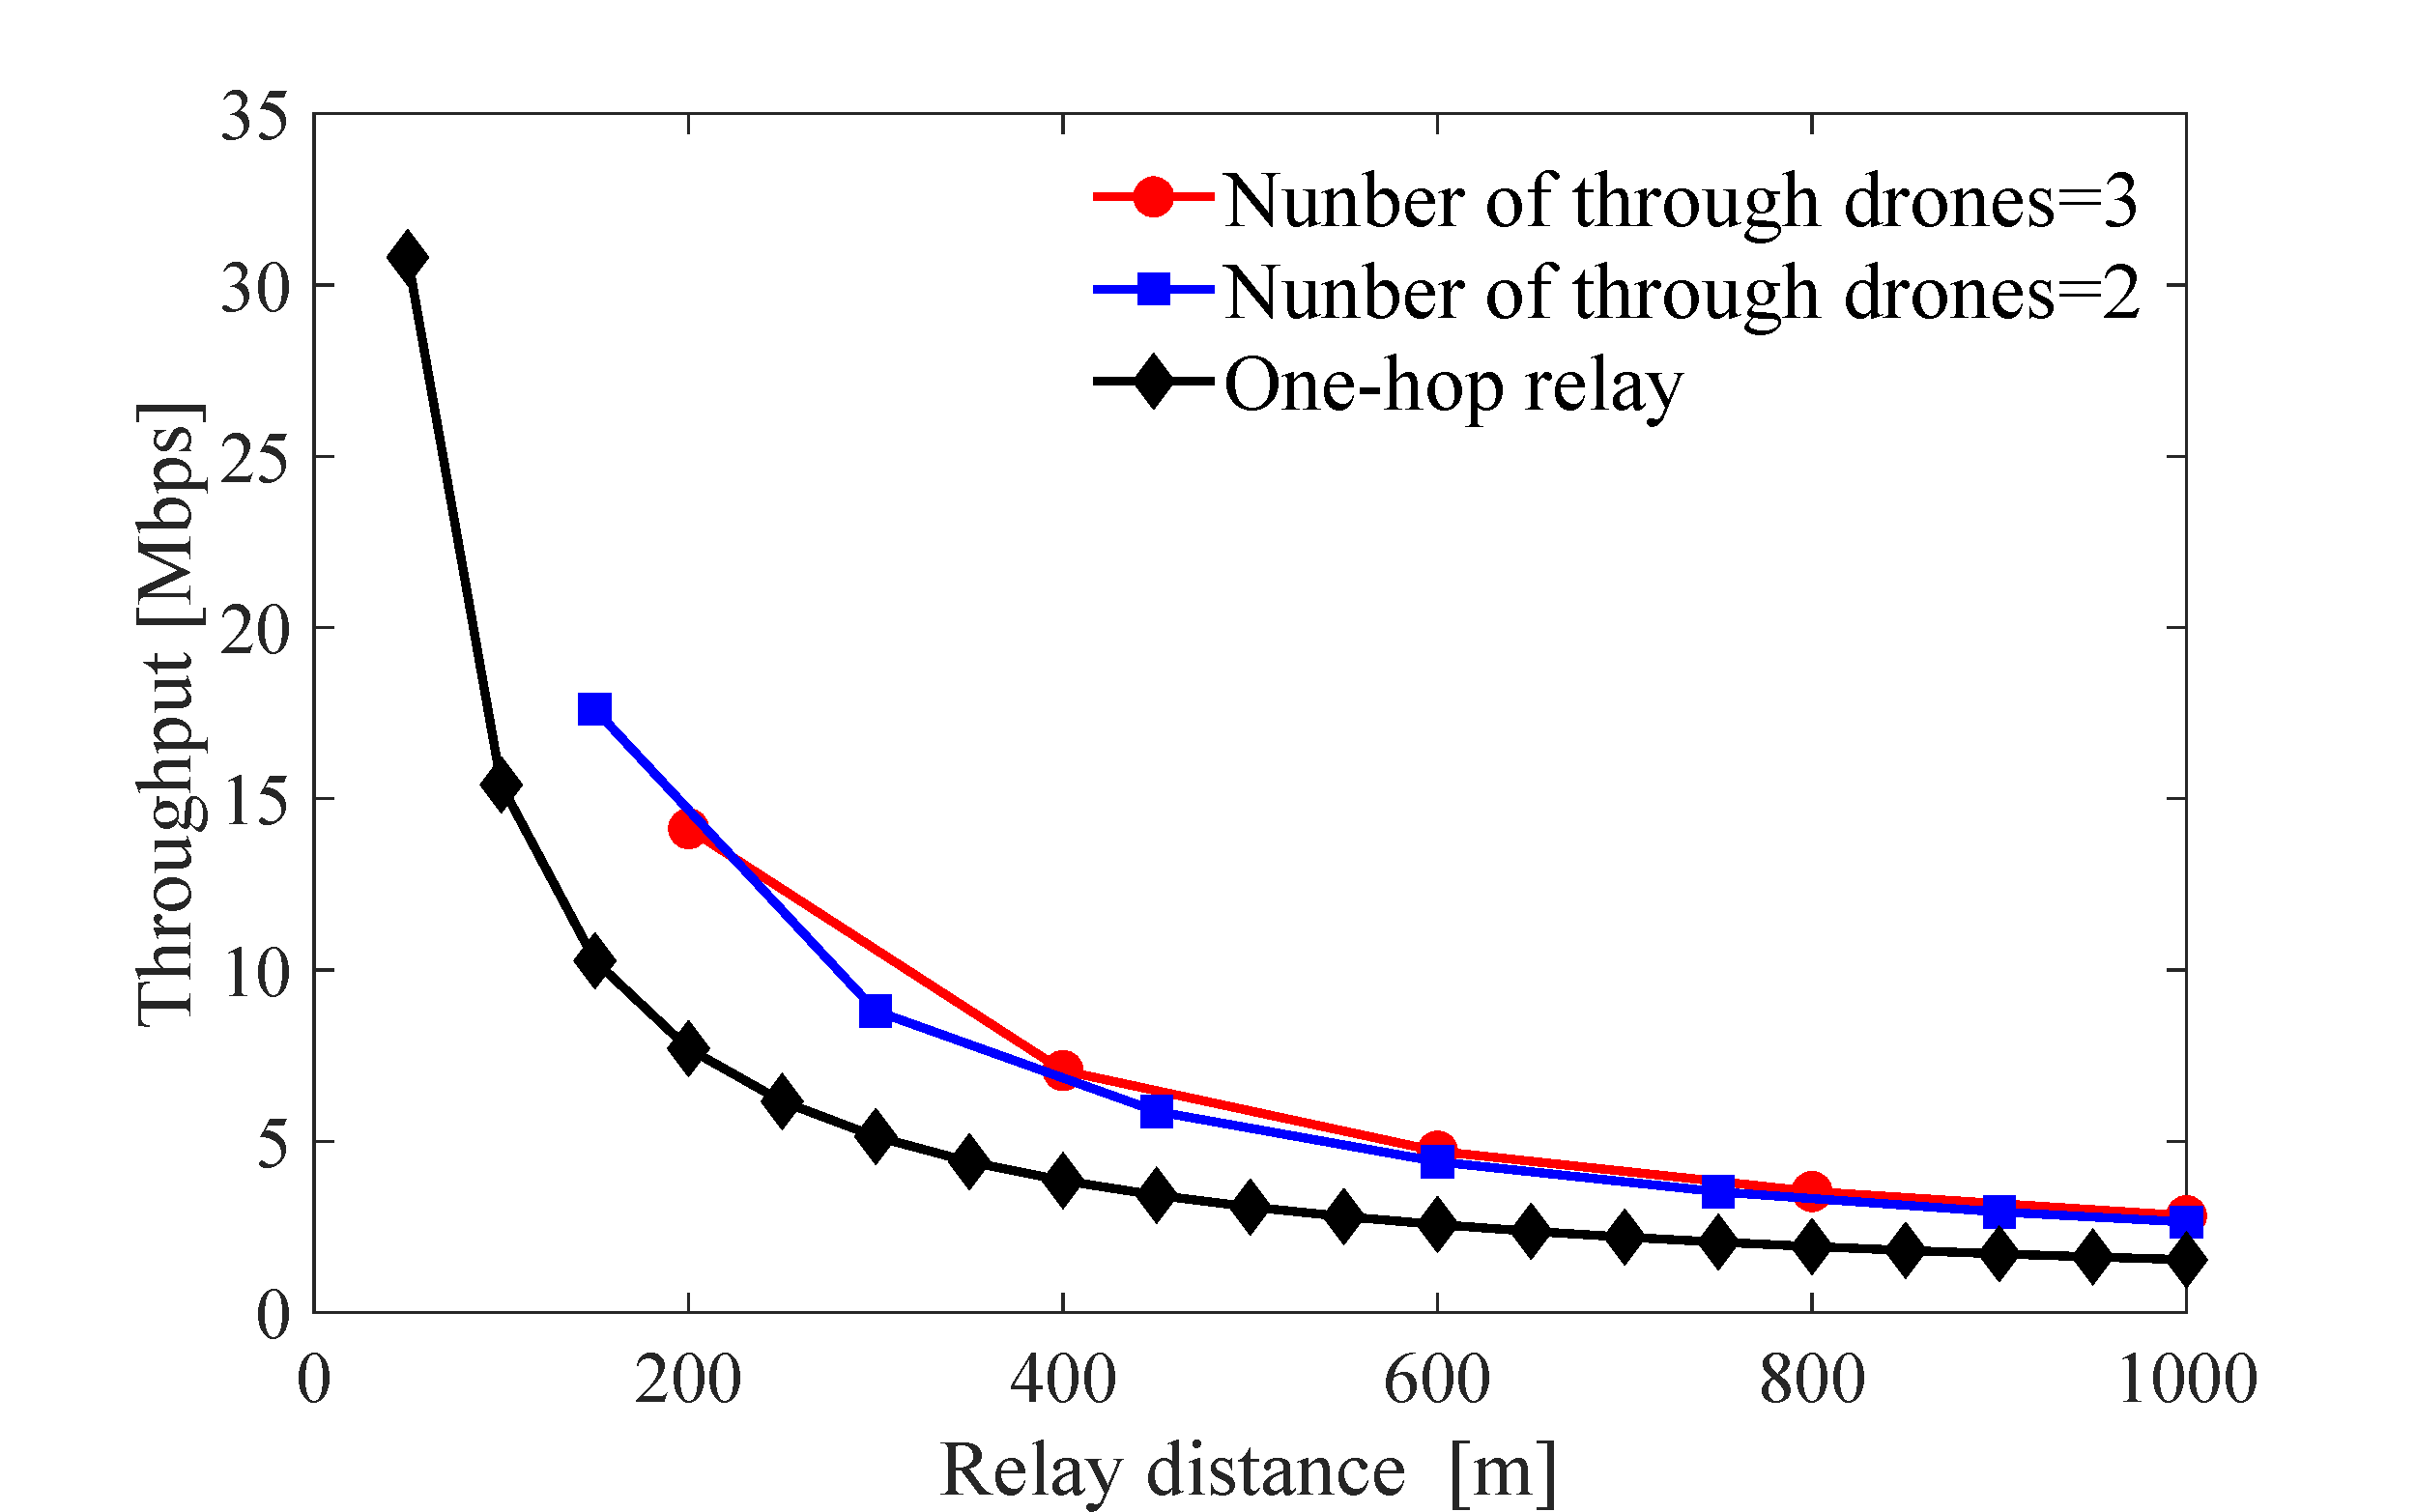
\includegraphics[width=\linewidth]{throughtput_vs_placement_50m_max_distance_3.pdf} % 図のファイル名を指定
  \caption{CTR方式と従来方式のスループット特性}
  \label{fig:throughput_through} % 参照用ラベル
\end{figure}
\begin{figure}[H]
  \centering
  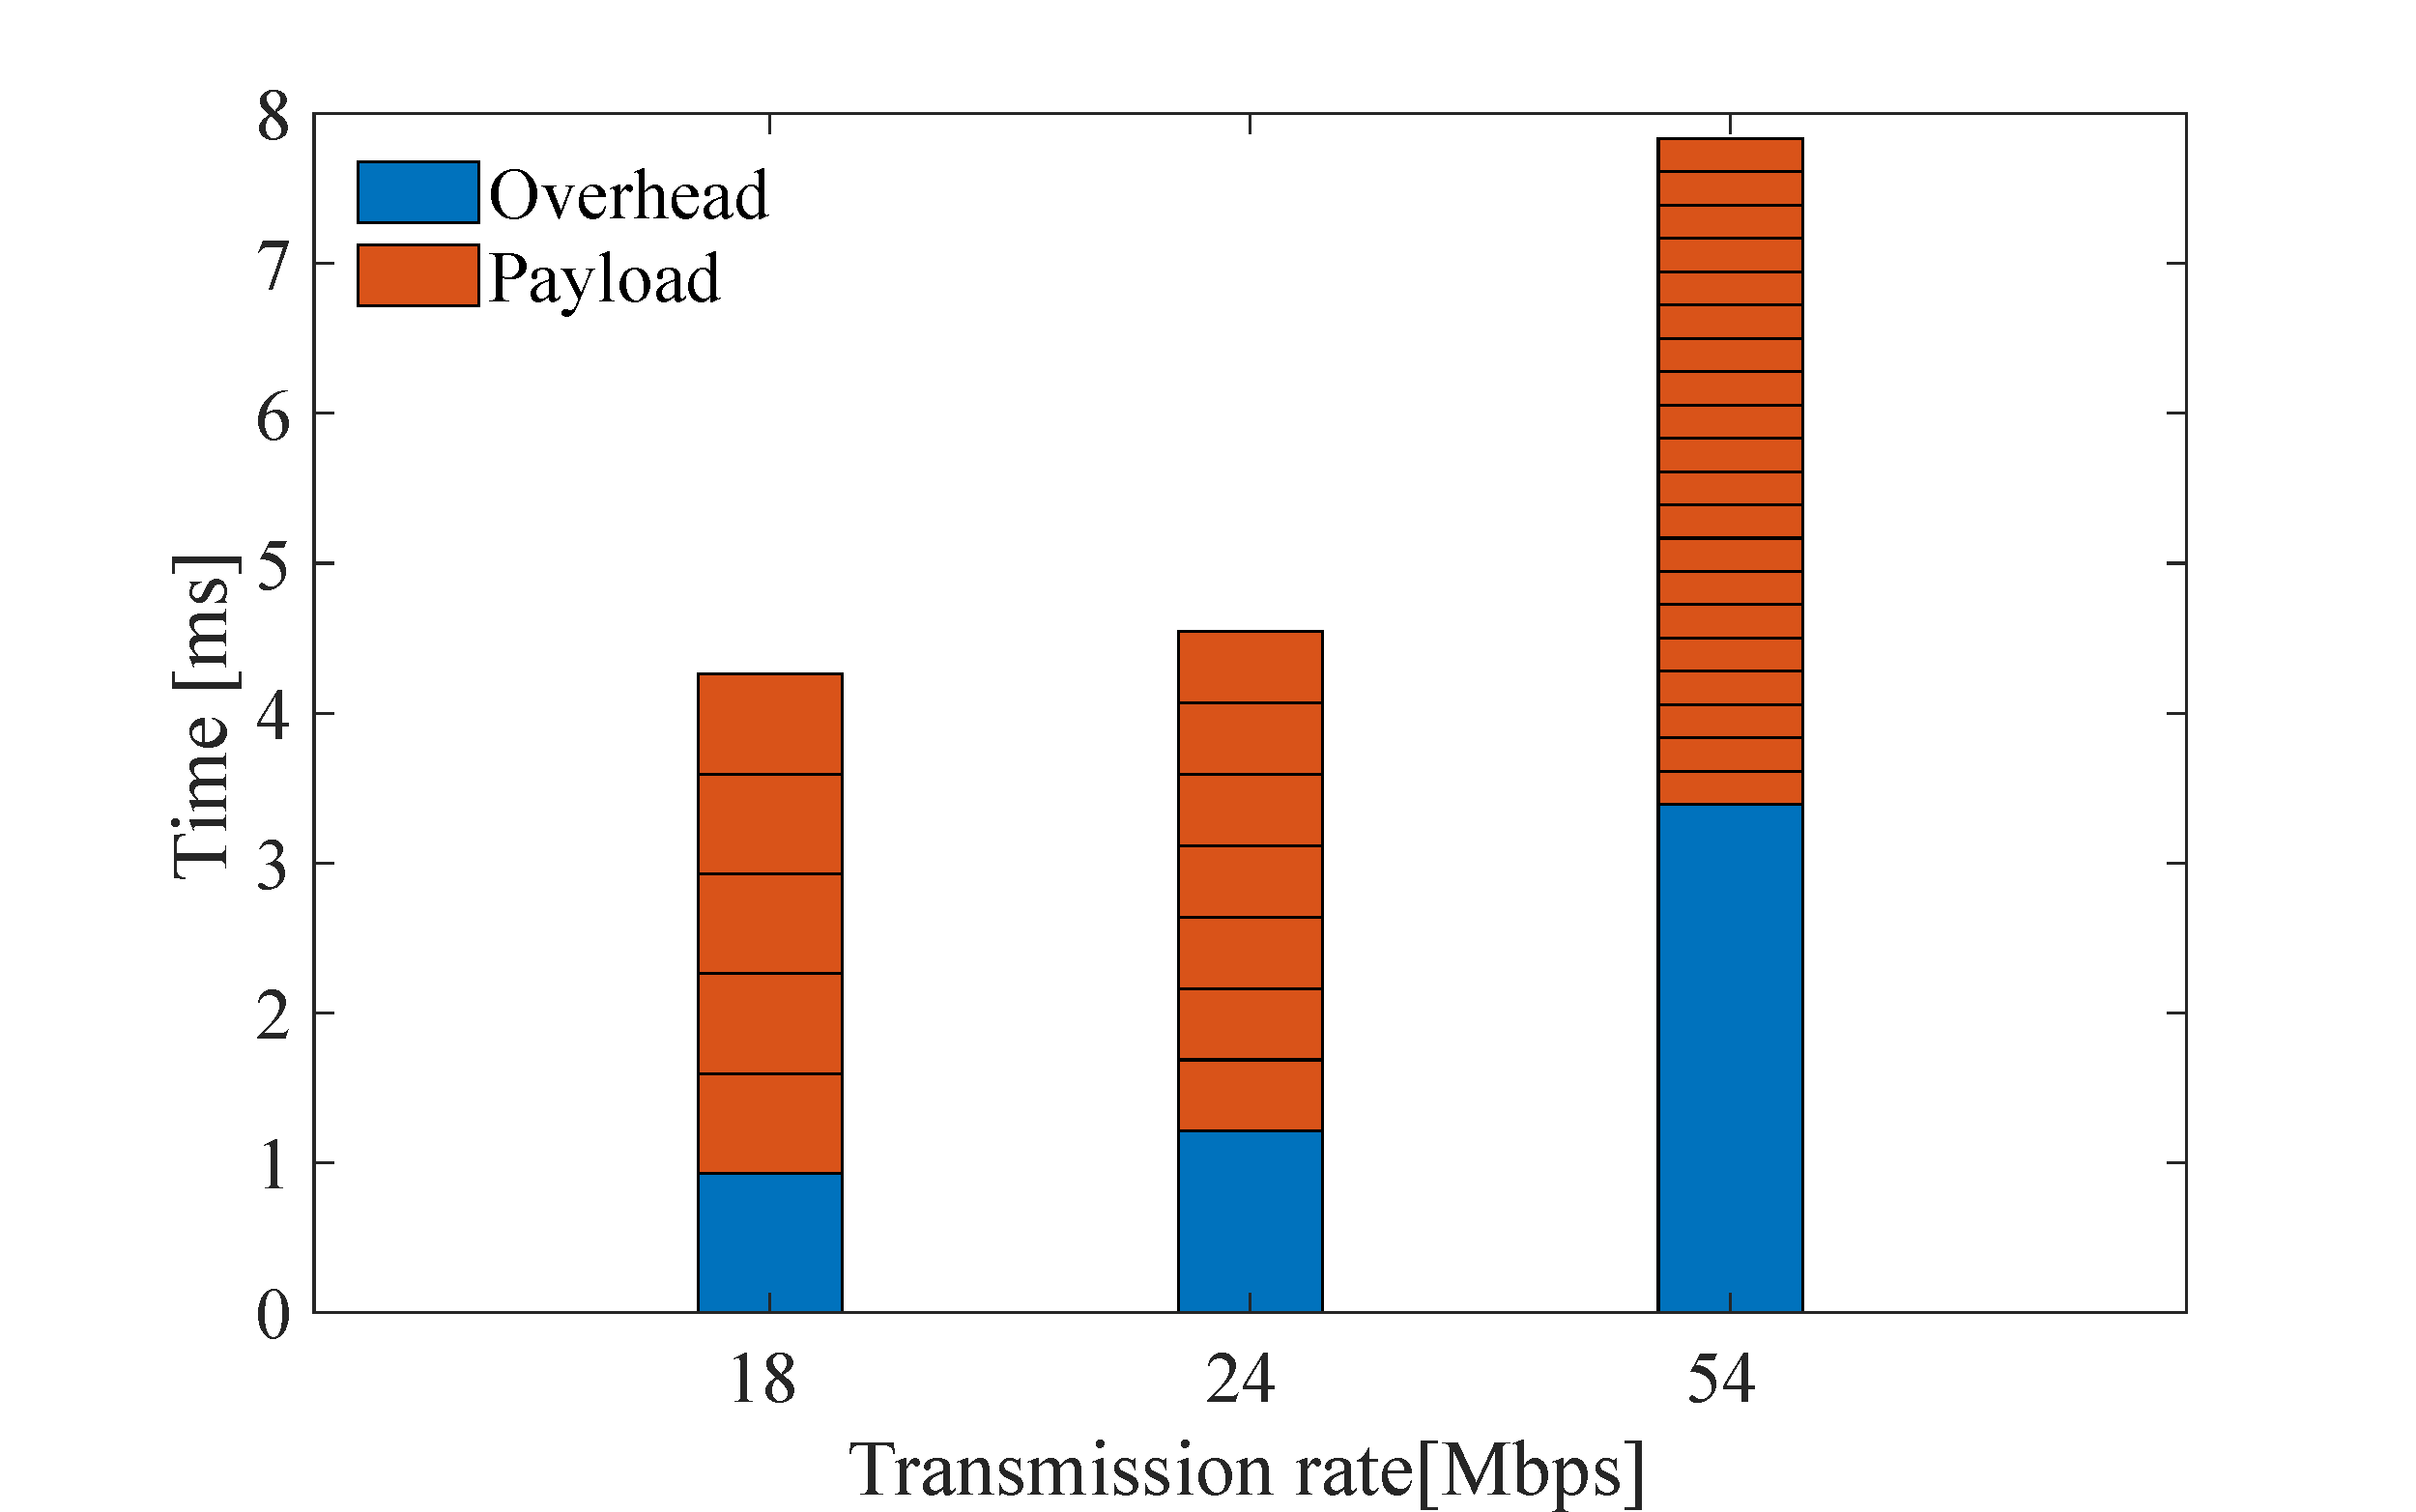
\includegraphics[width=\linewidth]{throughtput_vs_placement_50m_max_distance_3_2.pdf} % 図のファイル名を指定
  \caption{各伝送レートにおけるオーバヘッドとペイロードの時間}
  \label{fig:overhead_vs_paylord} % 参照用ラベル
\end{figure}

\clearpage
\subsection{誤りを生じる条件でのCTR方式の評価}
CTR方式のもう一つの特徴は,中継時に誤りが発生した場合,経路上の中継局が代替して中継を行うことにより,従来方式と比較してスループットが向上する点である.
この特性を,4.1の条件に基づいて従来方式と比較する.伝送レートは4.1の評価結果に基づき,18Mbpsとする.誤りが生じた際,従来方式ではフォールバック制御により伝送レートを1つ下の12Mbpsに変更し,その後の再送信は必ず成功するとする.これに対して,CTR方式では,誤りが生じた際,正しく受信できなかった中継局の1つ手前の中継局が必ず代替して中継できるとする.
この時パケットの誤り率を0\%から100\%まで変化させたときの従来方式とCTR方式の1000m地点での最終的なスループット特性を比較した.
\par
図\ref{fig:throughput_v3}に誤り率が変化したときスループットを示す.この結果から,誤り率が増加するほど従来方式よりスループットが高くなっているため,従来方式よりもCTR方式は干渉等によって局所的に誤り率が上がる条件(受信局)でも高効率に中継伝送が可能なことを確認した.
また,誤り率が増加するにつれて従来方式とCTR方式のスループットは減少しているが,CTR方式では誤り率によってスループットが緩やかに減少する部分がある.これはパケットの送信回数が関係していると考える.図\ref{fig:throughput_v3.1}には誤り率に対しての平均送信回数を示す.
図\ref{fig:throughput_v3.1}より従来方式の送信回数は誤り率に対して線形的に変化しているが,CTR方式の送信回数は線形的には変化していない.
これは,CTR方式で誤りが生じた際に,一つ前の中継局が通信を代替するからで,その結果,パケットの誤り率が増加しても送信回数の増加は緩やかに抑えられる.
この送信回数の抑制によりCTR方式のスループットは従来の方式と比較して減少が緩やかになる部分があると考えた.


\begin{figure}[H]
  \centering
  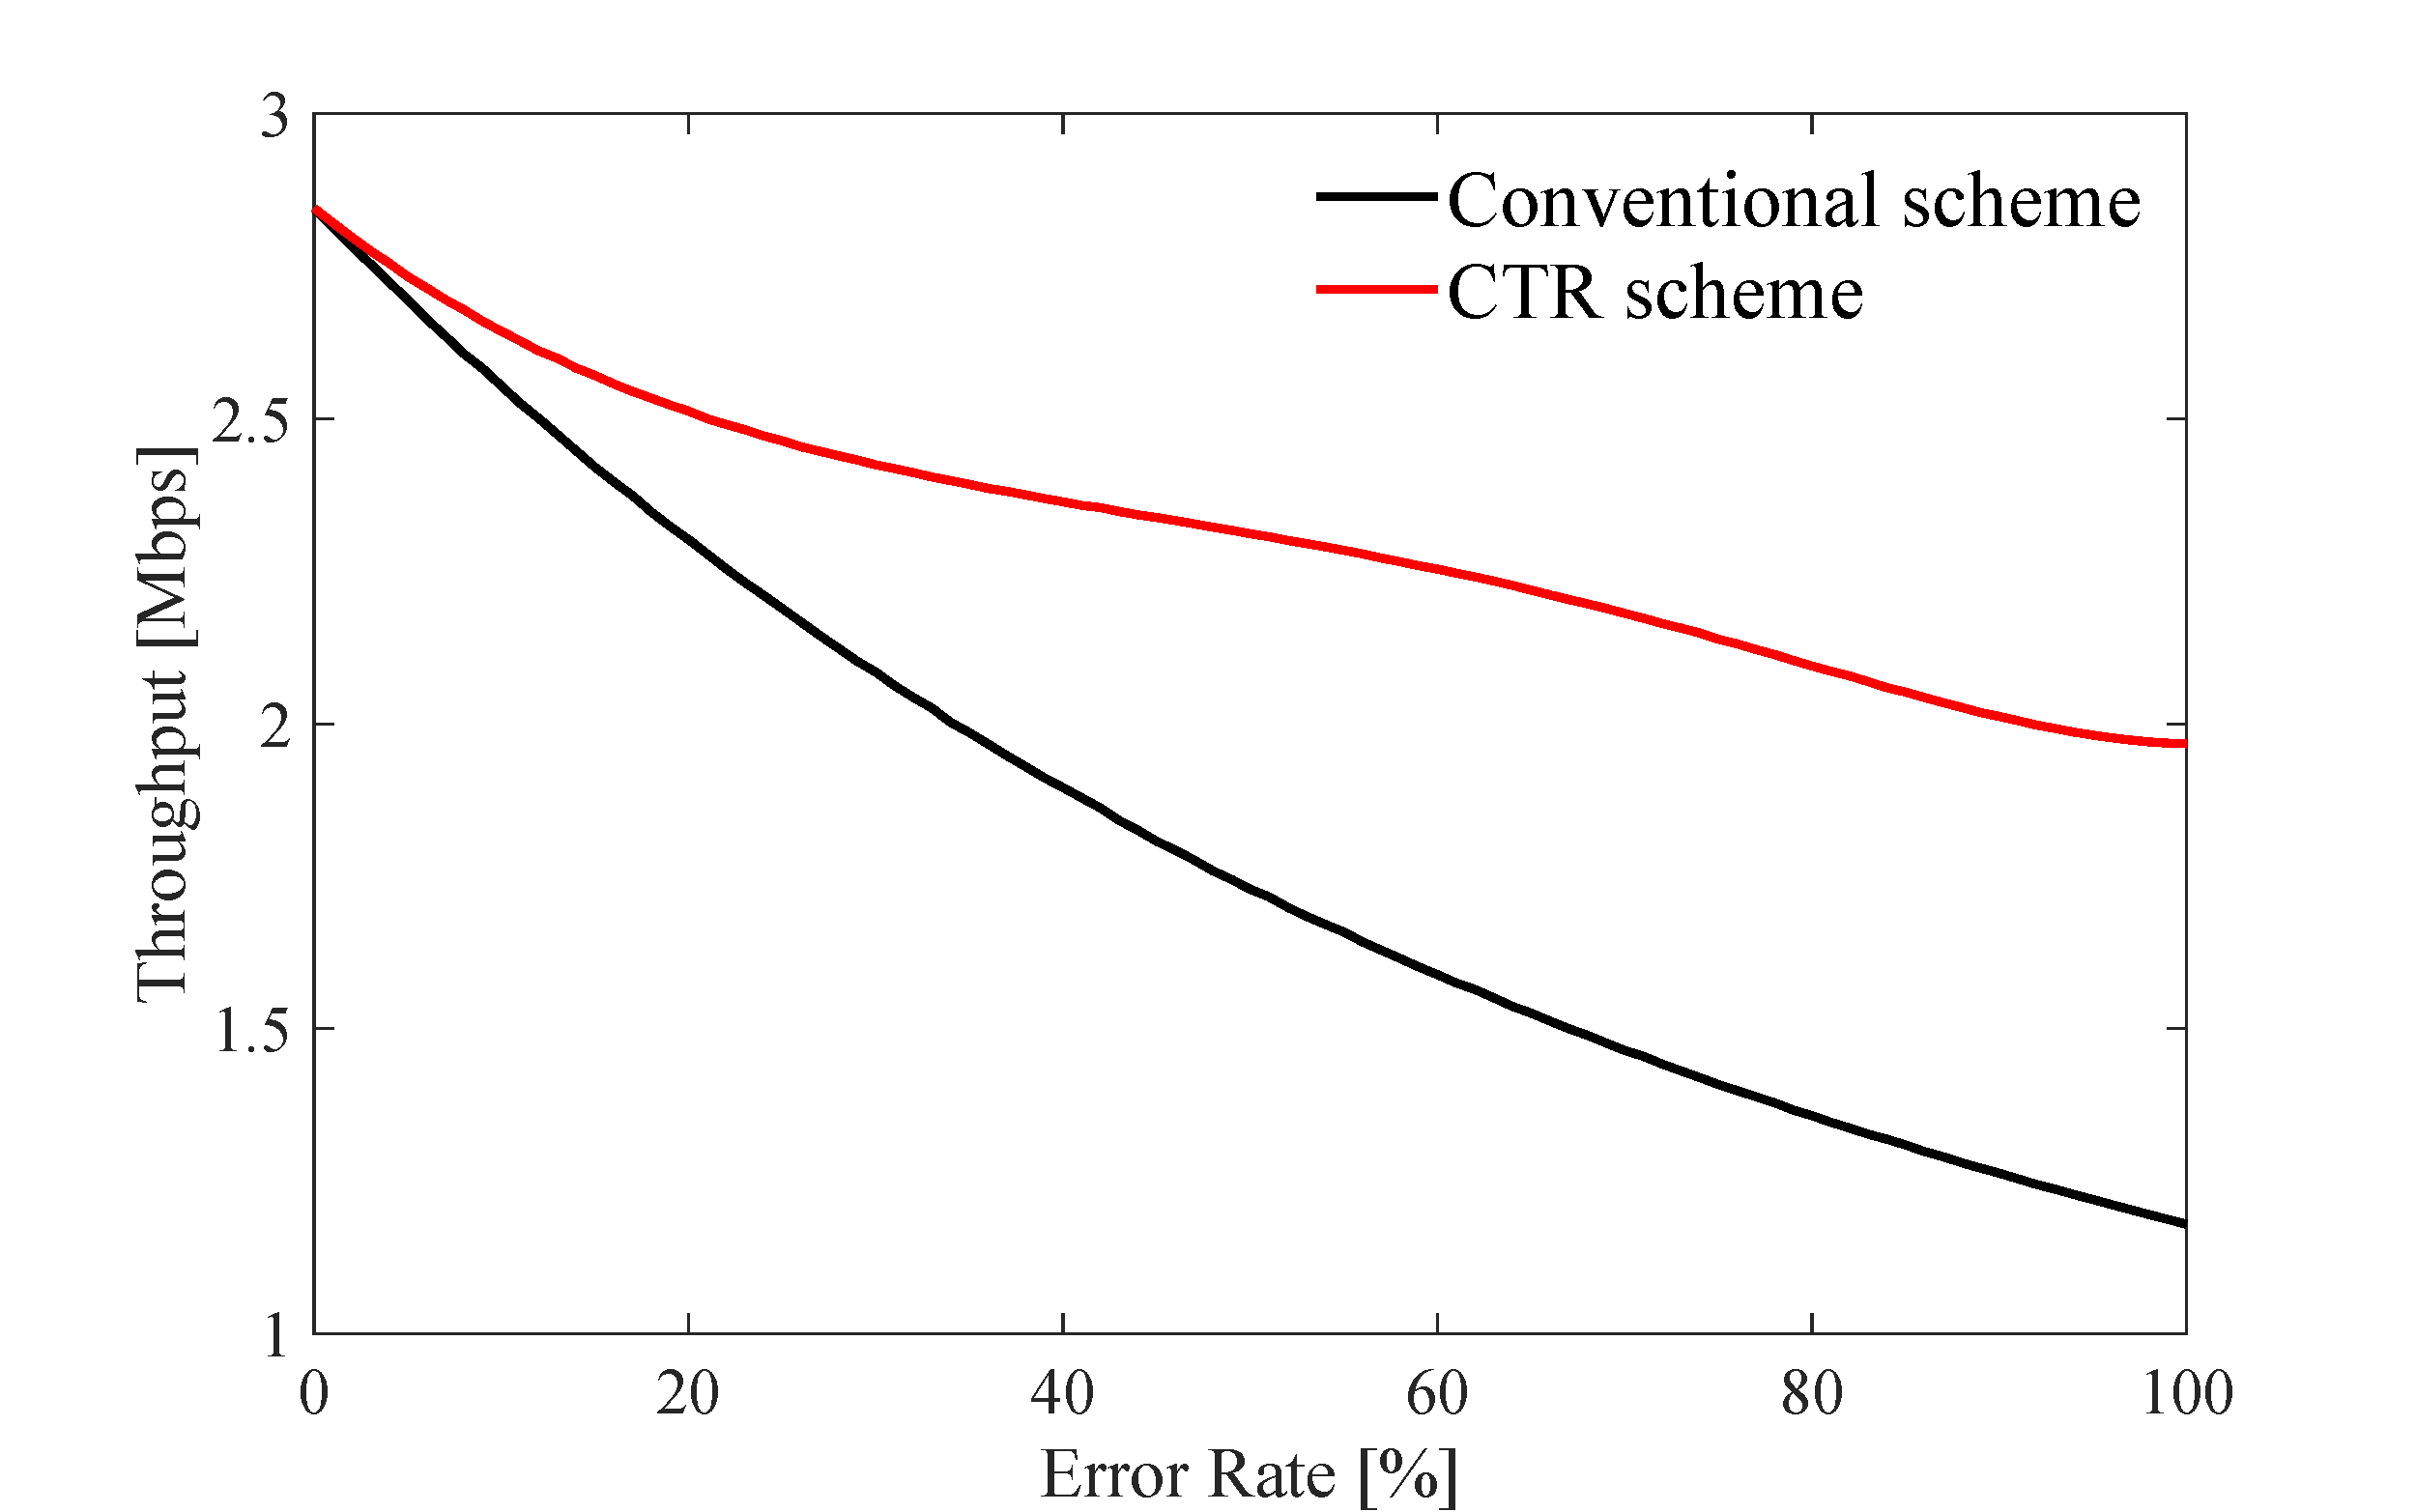
\includegraphics[width=\linewidth]{throughput_probabilistic_retry_v3.pdf} % 図のファイル名を指定
  \caption{誤り率に対するスループット特性}
  \label{fig:throughput_v3} % 参照用ラベル
\end{figure}
\begin{figure}[H]
  \centering
  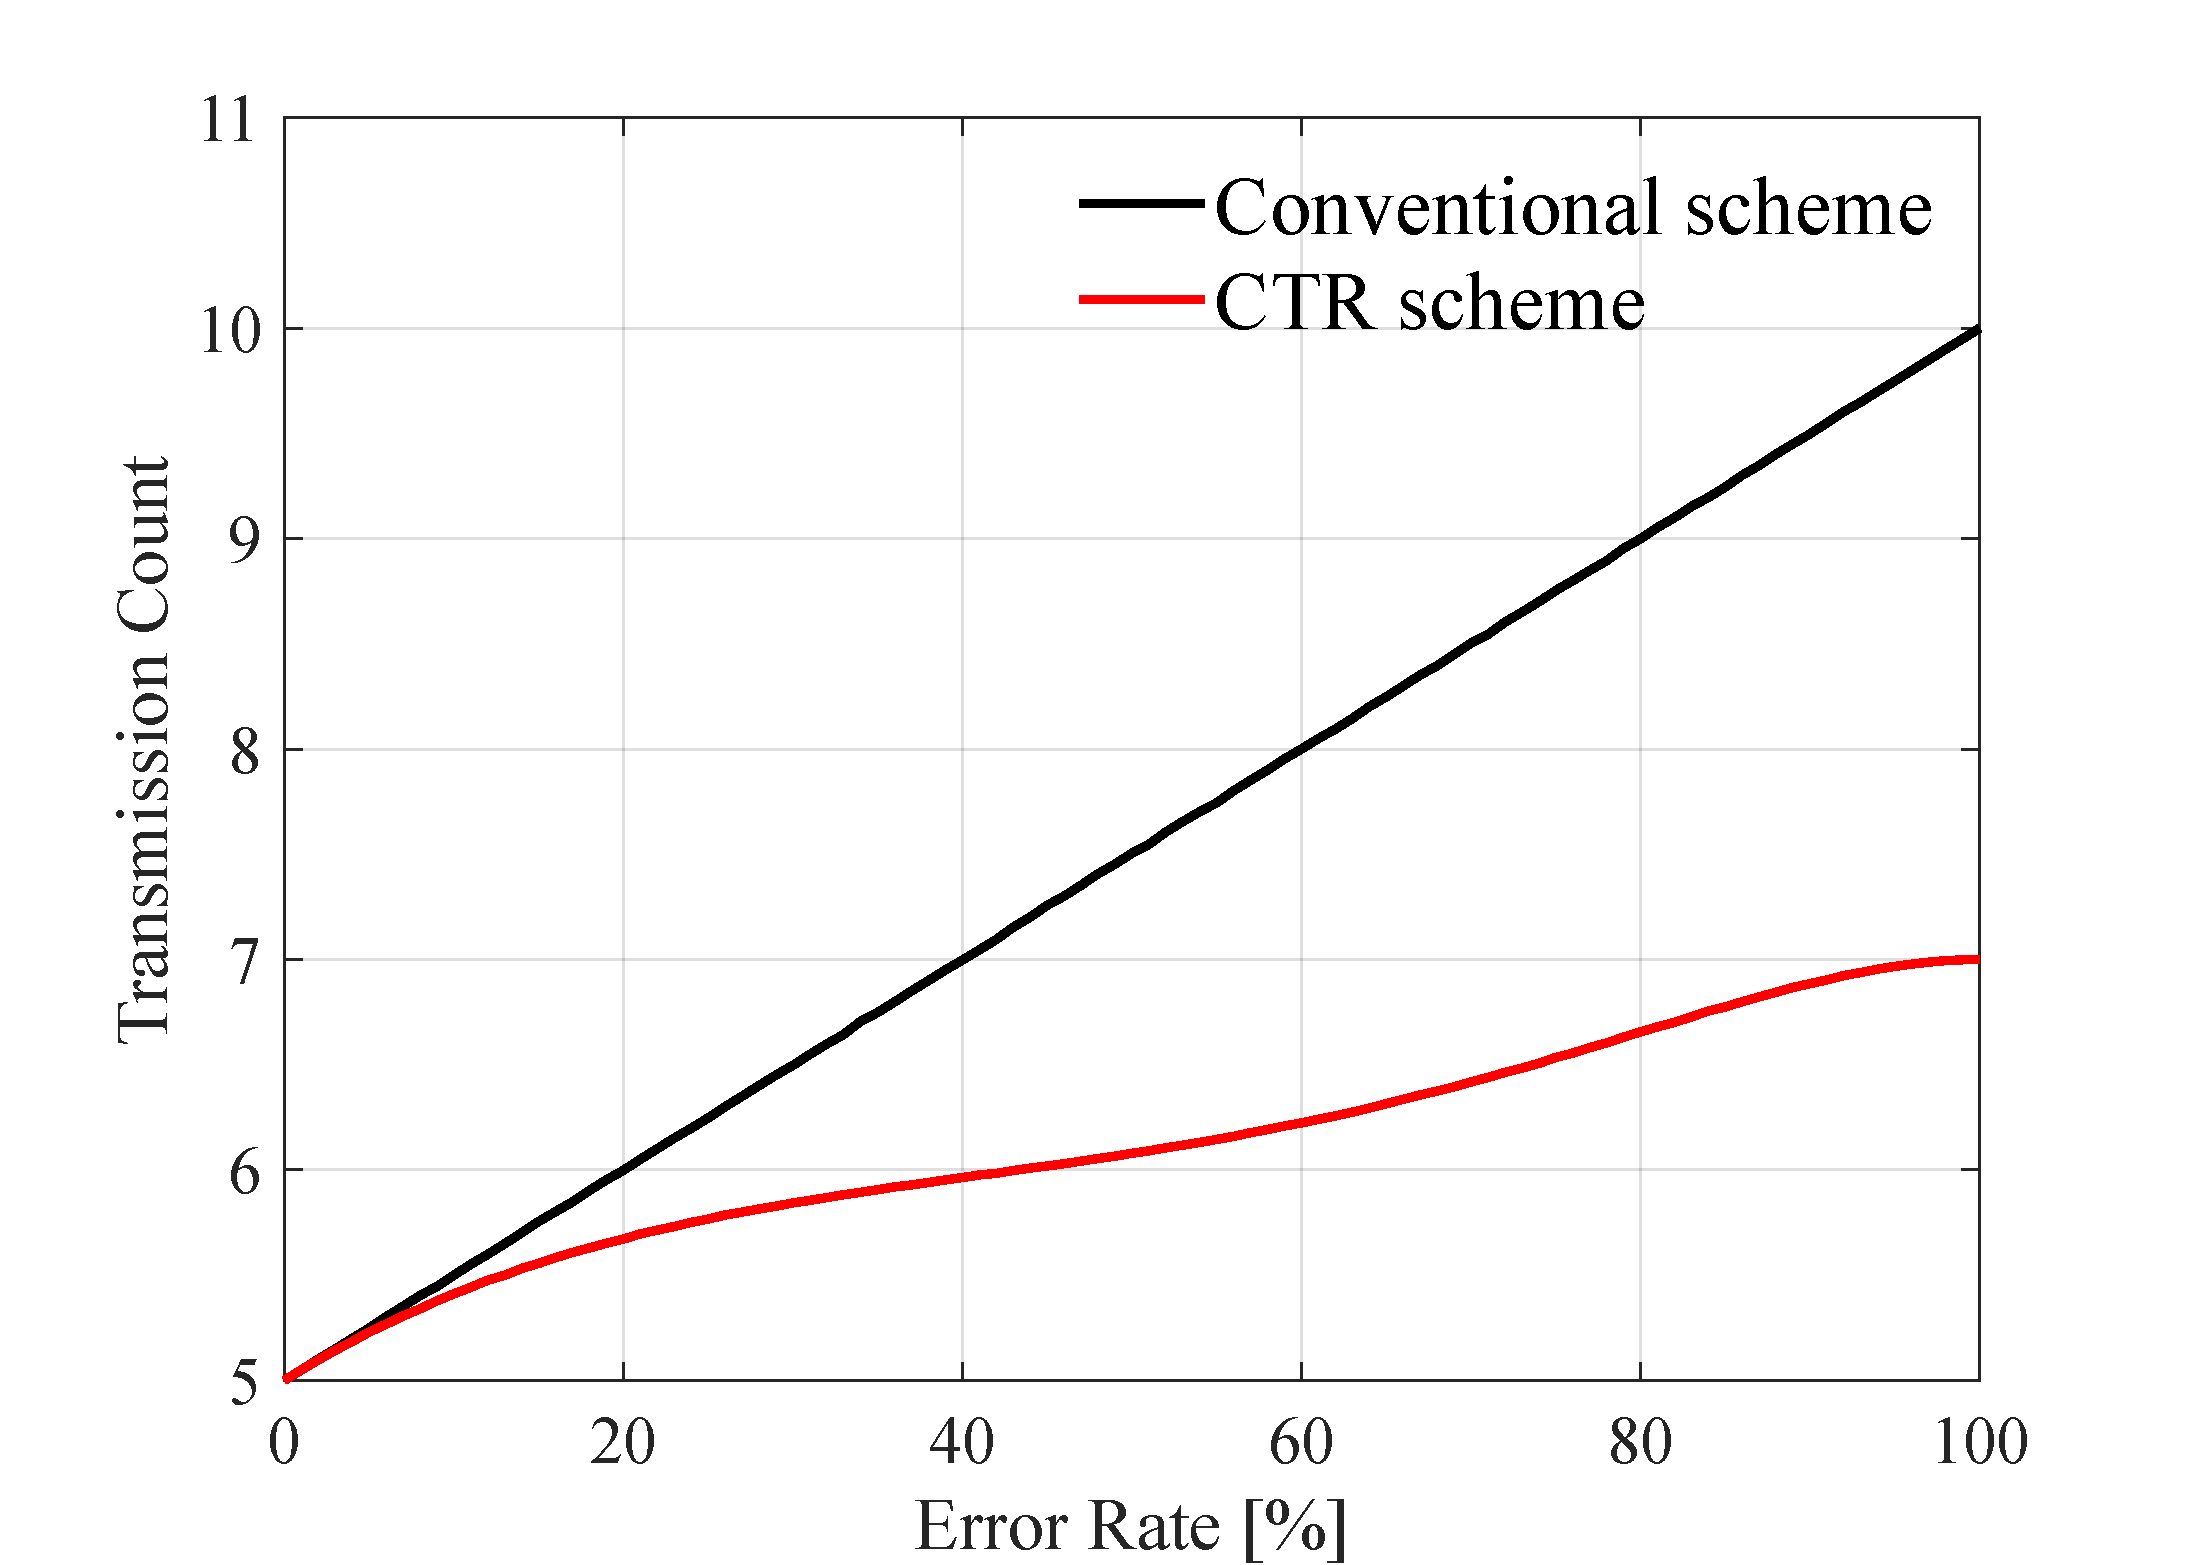
\includegraphics[width=\linewidth]{throughput_probabilistic_retry_v3.1.pdf} % 図のファイル名を指定
  \caption{誤り率に対しての平均送信回数の変化}
  \label{fig:throughput_v3.1} % 参照用ラベル
\end{figure}
\clearpage

% ******************************************************
% 6.おわりに
% ******************************************************
\section{おわりに}
本稿では,直線に配置されたドローン中継伝送におけるオーバリーチ干渉の影響を解決するために,送信信号の届く中継局まで一回で中継するCTR方式を検討した.
CTR方式と従来の方式で誤りが生じた場合と生じない場合のスループット特性を計算し比較した.
この結果からいずれの条件でもCTR方式はスループットが従来方式より高いことがわかった.
CTR方式では誤りが発生した場合においても再送信時にフォールバック制御による伝送レートの低下や中継時間の増加を防ぐことができるため、高効率な中継伝送が可能である.
\clearpage
\section{今後の課題}
\end{document}